\documentclass{scrartcl}

\usepackage[utf8]{inputenc}
\usepackage{amsmath}
\usepackage{amsthm}
\usepackage{amssymb}
\usepackage{geometry}
\usepackage{mathtools}
\usepackage{cancel}
\usepackage{xfrac}
\usepackage{siunitx}                                % for scientific notation \num{}
\usepackage{authblk}                                % for authors
\usepackage{tikz}                                   % for circled {}
\usepackage{systeme}                                % for system of equations bracket
\usepackage{verbatim}                               % for comment
\usepackage{xfp}                                    % for floating point operations in macros
\usepackage{graphicx}                               % for cropping the images
\usepackage{dsfont}                                 % for doublestroke fonts
\usepackage{float}
\usepackage{hyperref}                               % hyperlink
\usepackage[english]{babel}
\usepackage[square, numbers]{natbib}
\usepackage[nottoc, notlof, notlot]{tocbibind}     % Includes "References" in the table of contents
\usepackage{caption}
\usepackage{listings}
\usepackage{xparse}
\usepackage[none]{hyphenat}
\usepackage{subfig}


\bibliographystyle{abbrvnat}
% \captionsetup{justification=centering}
\lstset{language=python, keywordstyle={\bfseries \color{blue}}}

\NewDocumentCommand{\codeword}{v}{\texttt{\textcolor{blue}{#1}}}

\hypersetup{
	colorlinks=true, 
	citecolor=blue,
}

\AtBeginDocument{\renewcommand{\bibname}{References}}

\title{Video Prediction}
\subtitle{Independent Work Report (MAE 340, Spring 2021) \\ Advisor: Professor Olga Russakovsky}
\author{Matthew Coleman}
\date{April 26, 2022}

\begin{document}

\maketitle

\vspace{8cm}
\begin{center}
	\Large \textit{This project represents my own work, \\ in accordance with the University regulations.} \\
	\vspace{0.2cm}
	\large /s/Matthew Coleman
\end{center}
\normalsize

\newpage
\tableofcontents
\newpage

\section{Introduction}
\label{sec:intro}

While humans cannot perfectly predict the future, they are indeed capable of
inferring a great deal of information about near events in the future, and this
knowledge greatly aids them in planning out their actions, such as which
movements to take to reach a goal. This ability to forecast the future is a
direct result of an understanding of causality that is learned through
observation and interaction \cite{human_learning_sequences}.

Many human predictions are erroneous in major respects, but even humans least
adept at inferring far-off outcomes and consequences still are masters of
learning very near-term ones. For example, people generally have a good sense
for where a car will move in the street, or which direction a pedestrian may
continue walking. Even a young child can predict where to toss a football to a
moving receiver, and even this small knowledge reveals an infinite wisdom
compared to the most advanced video prediction methods.

The task of video prediction is comprised of several open challenges in
computer vision; it uses some of the most recent machine learning model
architectures that have been developed and it even contends directly with an
impossible task altogether, which is to predict the future. Although it is a
particularly confusing task, it also has the potential for immense impact and
immediate practical applications, such as in autonomous driving
\cite{eg_self_driving}, video interpolation \cite{eg_video_interp} and most
interesting in the context of this report, robotic control systems
\cite{eg_robot_control}.

This project will examine the current state-of-the-art in video prediction
machine learning models, report on several experiments carried out by
implementing and testing such a model on various existing datasets with varying
hyperparameters, and attempt to make meaningful conclusions about video
prediction based off of these results.

\section{The Task of Video Prediction}
\label{sec:task}

\newcommand{\Xseq}{$\boldsymbol{X} = \left( X_1 , X_2 , X_3 \cdots X_n \right)$}
\newcommand{\Yseq}{$\boldsymbol{Y} = \left( Y_1 , Y_2 , Y_3 \cdots Y_m \right)$}
\newcommand{\Yhatseq}{
	$\hat{\boldsymbol{Y}} = 
	\left( \hat{Y}_1 , \hat{Y}_2 , \hat{Y}_3 \cdots \hat{Y}_n \right)$
}

The task of video prediction is to construct an approximation for the
completion of a sequence of frames using only the initial sequence of frames.
Formally, given an ordered set of $n$ image frames \Xseq, the task is to
predict the immediately following $m$ frames of the sequence \Yseq, each of
which having the same dimensions, for example with $c$ channels, height $h$,
and width $w$. At each inference in training, the model predictions \Yhatseq,
with the same dimensions as the inputs, are conditioned on the input sequence
$\boldsymbol{X}$, and the model weights are updated typically by the gradient
of a loss function computed between the predictions and ground truth sequence
$\boldsymbol{Y}$ directly. Critically, since there is no human intervention or
labeling required for the model to do this, and models typically are able to
learn from the implicit temporal organiziation of the video data, video
prediction is a self-supervised task \cite{video_prediction_survey}.

% A great deal of discussion in video prediction research centers around exactly
% how these predictions are computed, specifically by testing different model
% architectures, loss functions, and training approaches, however, there is also
% a good amount of disagreement on how model predictions are actually evaluated.
% For example, models trained using pixel-wise loss functions such as MSE will
% typically prefer blurrier predictions in order to capture the underlying
% stochasticity of the data, whereas GANs will prefer to produce more realistic
% data, even if the predictions are further off the mark.

\newpage
\section{Families of Prediction Models}
\label{sec:families}

Modern video prediction models tend to adopt several canonical architectures,
which are normally simple and easily generalizable for specific tasks, such
that they can be used as building blocks or blueprints within larger
architectures. Understanding what each architecture seeks to do on a high level
is imperative to understanding what kind of output one should expect from the
model or how to debug and improve it, and research implementations make use
of these basic concepts in different ways.

For example, RNNs and generative networks are each successful and well-tested
paradigms used in many other machine learning domains outside of computer
vision, but they are especially utilized within video prediction because of
their key properties and strengths, particularly of RNNs to work on
time-sequential data and of generative networks to ``imagine'' new data within
a distribution. These paradigms are used extensively in Convolutional LSTM
(ConvLSTM), FutureGAN \cite{futuregan}, and SAVP models \cite{savp} for video
prediction, as well as many other models in cutting-edge research. A short
description of each family and its relevance to video prediction is given
below:

\subsection{Recurrent Neural Networks}
\label{subsec:rnn}

Formally, a Recurrent Neural Network (RNN) is the end-result of a mathematical
analysis of a nonlinear first-order non-homogeneous ordinary differential
equation describing the evolution of a state signal $s$ as a function of time,
along with an input signal $x$. The canonical statement of an RNN is given
below in the form of a system of discrete Delay Differential Equations (DDE)
\cite{rnn_and_lstm_fundamentals}:

\begin{equation}
	\begin{split}
		s_t & = W_s s_{t - 1} + W_r r_{t - 1} + W_x x_t + \theta_s \\
		r_t & = G ( s_t )
	\end{split}
	\label{eq:rnn_canonical}
\end{equation}

With $W_s$, $W_r$, and $W_x$ as weights which are either multiplied or
convolved with their respective signals, and $\theta_s$ as a bias term
which is typically added in element-wise fashion to $s$. This equation
also includes the read-out or output signal $r$, which is the activation
$G(z)$ of the state signal, and can be seen as the ``output'' of the network.
All together, this equation describes all of the moving parts of an RNN.

As a toy example (and ignoring some technical tricks that would be required to
make this actually happen), a network of this type should be capable of
transcribing seqeunces of a lecture by evaluating discrete audio samples
recorded from the event and outputting the spoken words in text form
\cite{rnn_and_lstm_fundamentals}. Another extremely common application of
vanilla RNNs is machine translation, in which the input sequence is text in one
language and the output is meant to be the translation of that text into
another language.

A more easily understandable depiction of the RNN described in Equation
\ref{eq:rnn_canonical} can be found in Figure \ref{fig:rnn_arch}. This figure
also shows the ``unfolding'' or ``unrolling'' of the model, which is just a way
of seeing each time-step of the state signal $s_t$, input signal $x_t$, and
ouput signal $r_t$ (here replaced by $\hat{y}_t$, denoting the network
inferences) as they are produced over time.

\begin{figure}[H]
	\begin{center}
		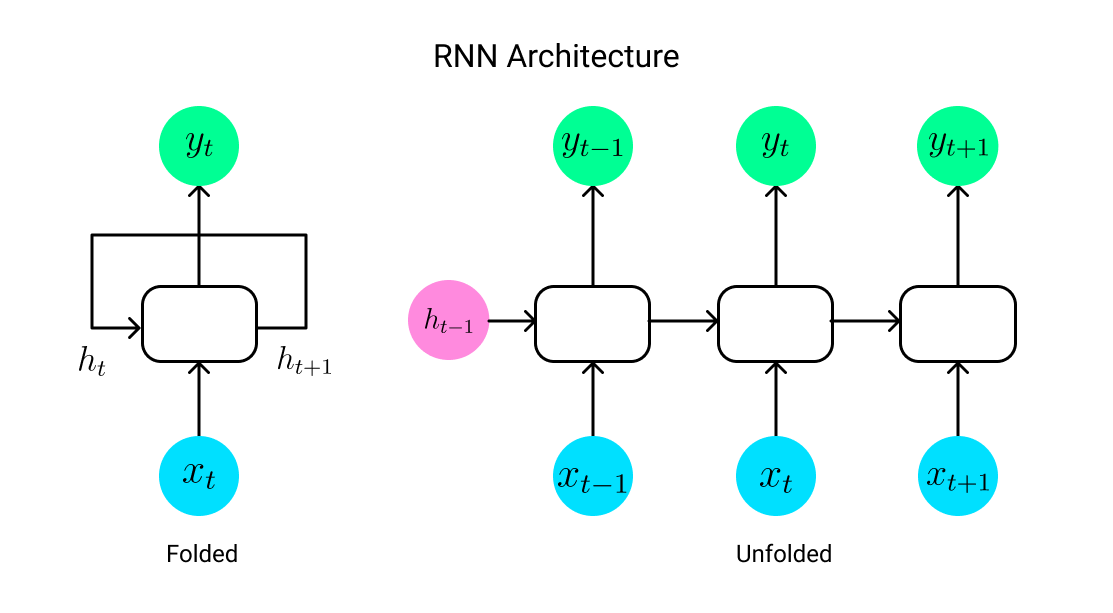
\includegraphics[width=1\textwidth]{figures/rnn_arch.png}
	\end{center}
	\caption{RNN Architecture}
	\label{fig:rnn_arch}
\end{figure}

RNNs are generally trained using a techinque called Backpropagation Through
Time (BPTT), in which the gradient of a loss function taken between model
outputs and ground truth labels at a certain instance in time is used to update
the model parameters recursively through the history of the model, using the
chain rule. In this way, RNN models trained over long sequences have their
parameters updated by the product of many Jacobian matrices, which, just like a
product of many real numbers, can vanish or explode very easily
\cite{rnn_training_challenges}. For this reason, along with several others
having to do with the long-term stability of RNNs, the Long Short-Term Memory
(LSTM) cell was developed with nonlinear, data-dependent controls in the form
of several ``gates'' that control input to and output from the cell's state
\cite{rnn_and_lstm_fundamentals}.

\subsection{Long Short-Term Memory (LSTM) Cell}
\label{subsec:lstm}

The changes described in the following section take the form of a modified
system of equations \cite{rnn_review}: 

\newcommand{\csquig}{\tilde{c}}

\begin{equation}
	\begin{split}
		f_t           & = \sigma ( W_{fh} h_{t - 1} + W_{fx} x_t + b_f ) \\
		i_t           & = \sigma ( W_{ih} h_{t - 1} + W_{ix} x_t + b_i ) \\
		\csquig_t     & = \tanh ( W_{\csquig h} h_{t - 1} + W_{\csquig x} x_t + b_{\csquig} ) \\
		o_t           & = \sigma ( W_{oh} h_{t - 1} + W_{ox} x_t + b_o ) \\
		c_t           & = f_t \circ c_{t - 1} + i_t \circ \tilde{c}_t \\
		h_t           & = o_t \circ \tanh ( c_t )
	\end{split}
	\label{eq:lstm_canonical}
\end{equation}

The key differences in the LSTM are the four gates denoted by $f$, $i$,
$\tilde{c}$, and $o$. Other than these, the cell state $c$ and output $h$ are
analogous to the original RNN definition. Now, the input and output gates are
able to ``learn'' how to add information to the cell state or take information
for inferences, and the forget gate is able to remove information from the cell
state entirely. To see how this is done, recall that the sigmoid funtion
$\sigma (z)$ has an output range of $(0, 1)$, meaning that element-wise
multiplication by embeddings activated by sigmoid can minimize and essentially
nullify the cell state. In the input gate, this same technique is applied for
$i$ onto $\tilde{c}$, and in the output gate it is applied by $o$ onto $c$,
meaning that $i$ decides what from $h_{t - 1}$ is allowed into the cell state
and $o$ decides what from $c_{t - 1}$ is allowed out of the cell state into the
inference. A diagram of these connections is shown in Figure
\ref{fig:lstmcell_arch}.

\begin{figure}[H]
	\begin{center}
		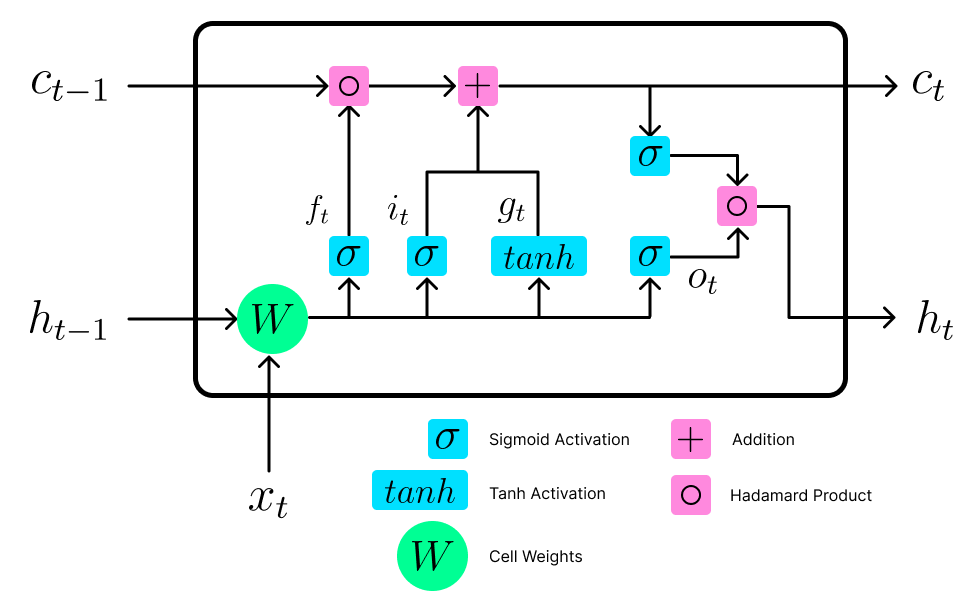
\includegraphics[width=1\textwidth]{figures/lstmcell_arch.png}
	\end{center}
	\caption{LSTM Cell Architecture}
	\label{fig:lstmcell_arch}
\end{figure}

In this way, LSTM cells are capable of mitigating some of the drawbacks of RNNs
such as vanishing and exploding gradients, and they are capable of learning how
to make good inferences for very different sequences. In other words, they are
better able to approximate both $y ( t_1 )$ and $y ( t_2 \gg t_1 )$ using the
same parameters.

Now that some of the general architectures and methodologies are laid out,
however, the question still remains of how these models actually predict the
continuation $\boldsymbol{Y}$ of a sequence of frames $\boldsymbol{X}$ with any
sort of accuracy. In order to do this, one final methodology must be examined,
namely Sequence to Sequence (Seq2Seq) learning, which will lead to the final
implementation of a Convolutional LSTM used for experimentation in this
project.

\subsection{Sequence To Sequence Learning}
\label{subsec:seq2seq}

Seq2Seq learning is only a slight modification to the original usage of RNNs,
but they represent an elegant solution to a classical shortcoming of most Deep
Neural Networks (DNNs), which is that they can only be applied to problems in
which inputs and outputs can fit into fixed, discretized, vectors, and
therefore must be of a certain length or size. Seq2Seq learning solves this
problem for video prediction as well as many other tasks by using 2 LSTMs: an
encoder to read the sequence and learn to create an embedding vector, and a
decoder, which is passed the embedding vector and learns to generate the
predicted sequence \cite{seq2seq_original}. A diagram of this procedure is
shown in Figure \ref{fig:seq2seq_arch}.

\begin{figure}[H]
	\begin{center}
		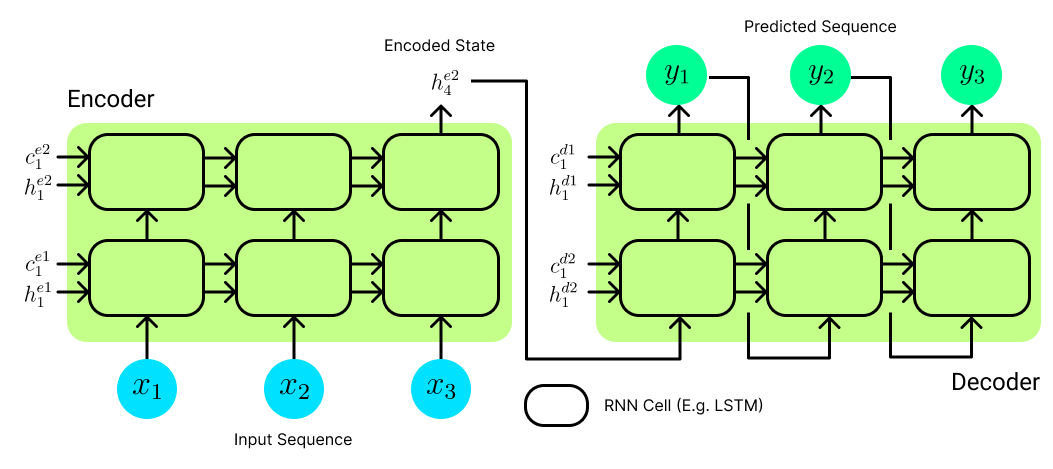
\includegraphics[width=1\textwidth]{figures/seq2seq_arch.png}
	\end{center}
	\caption{Seq2Seq Architecture}
	\label{fig:seq2seq_arch}
\end{figure}

The diagram shows how the input sequence $x$ is fed into the encoder LSTM for 3
steps (in practice this can be any length), how the encoder generates an
embedding vector $h_4$ which is passed to the decoder as an input, and how the
decoder generates the predicted sequence by passing the predicted output
$\hat{y}_{t}$ back into itself at the next time step as an input, continuing
until all predicted frames are generated.

This diagram also shows two layered LSTM cells, which is another key
modification used in this project's implementation. Note that each layer has
it's own states $h$ and $c$, and at each time step, the cells pass their $h$
embedding up to the next cell as an input. Deep, multilayered LSTMs have been
shown to significantly outperform shallow LSTMs for language translation
\cite{seq2seq_original}, however, this project will also analyze the effect of
depth on LSTM inferences for video prediction. 

In sum, these are the main methods used in this report's implementation of an
LSTM model for video prediction, which is discussed in further detail in the
following section.

% \subsection{Generative Models}
% \label{subsec:generative}
%
% \begin{figure}[H]
% 	\begin{center}
% 		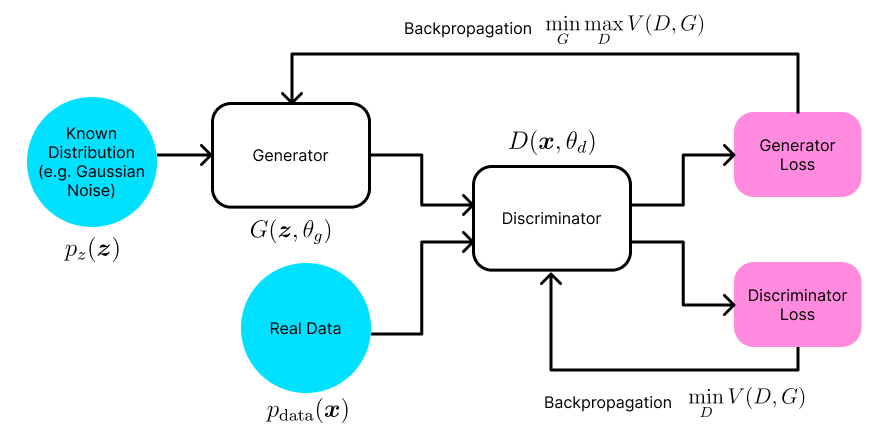
\includegraphics[width=1\textwidth]{figures/gan_arch.png}
% 	\end{center}
% 	\caption{General GAN Architecture}
% 	\label{fig:gan_arch}
% \end{figure}
%
% Generative neural networks (for example, GANs) consist of mostly the same
% architecture as discriminative neural nets, such as the ones which are
% classically used for image classification. While discriminative nets seek to
% learn the conditional probability $p(y \mid x)$ of an input $x$ belonging to a
% particular class $y$, generative nets seek to learn the conditional probability
% distribution $p(x \mid y)$ of an input data given the output, allowing them to
% make inferences in the form of ``imagined'' data that might belong to the same
% distribution as $x$ \cite{gan_original}. In short, discriminative models would
% look at many Van Gogh paintings and fakes in order to learn to differentiate
% between them, and generative models would look at many Van Gogh paintings in
% order to learn how to paint like Van Gogh.
%
% In practice, this is done by passing a low-dimensional embedding vector from a
% known latent distribution (such as the kind that may come as an activation from
% a discriminative net) through a typical network in reverse, generating an
% upscaled output in the same shape as the targeted learning data.

% \section{Video Prediction Models}
% \label{sec:families}

% \subsection{Convolutional LSTM}
% \label{subsec:conv_lstm}
%
% \subsection{FutureGAN}
% \label{subsec:futuregan}
%
% \begin{figure}[H]
% 	\begin{center}
% 		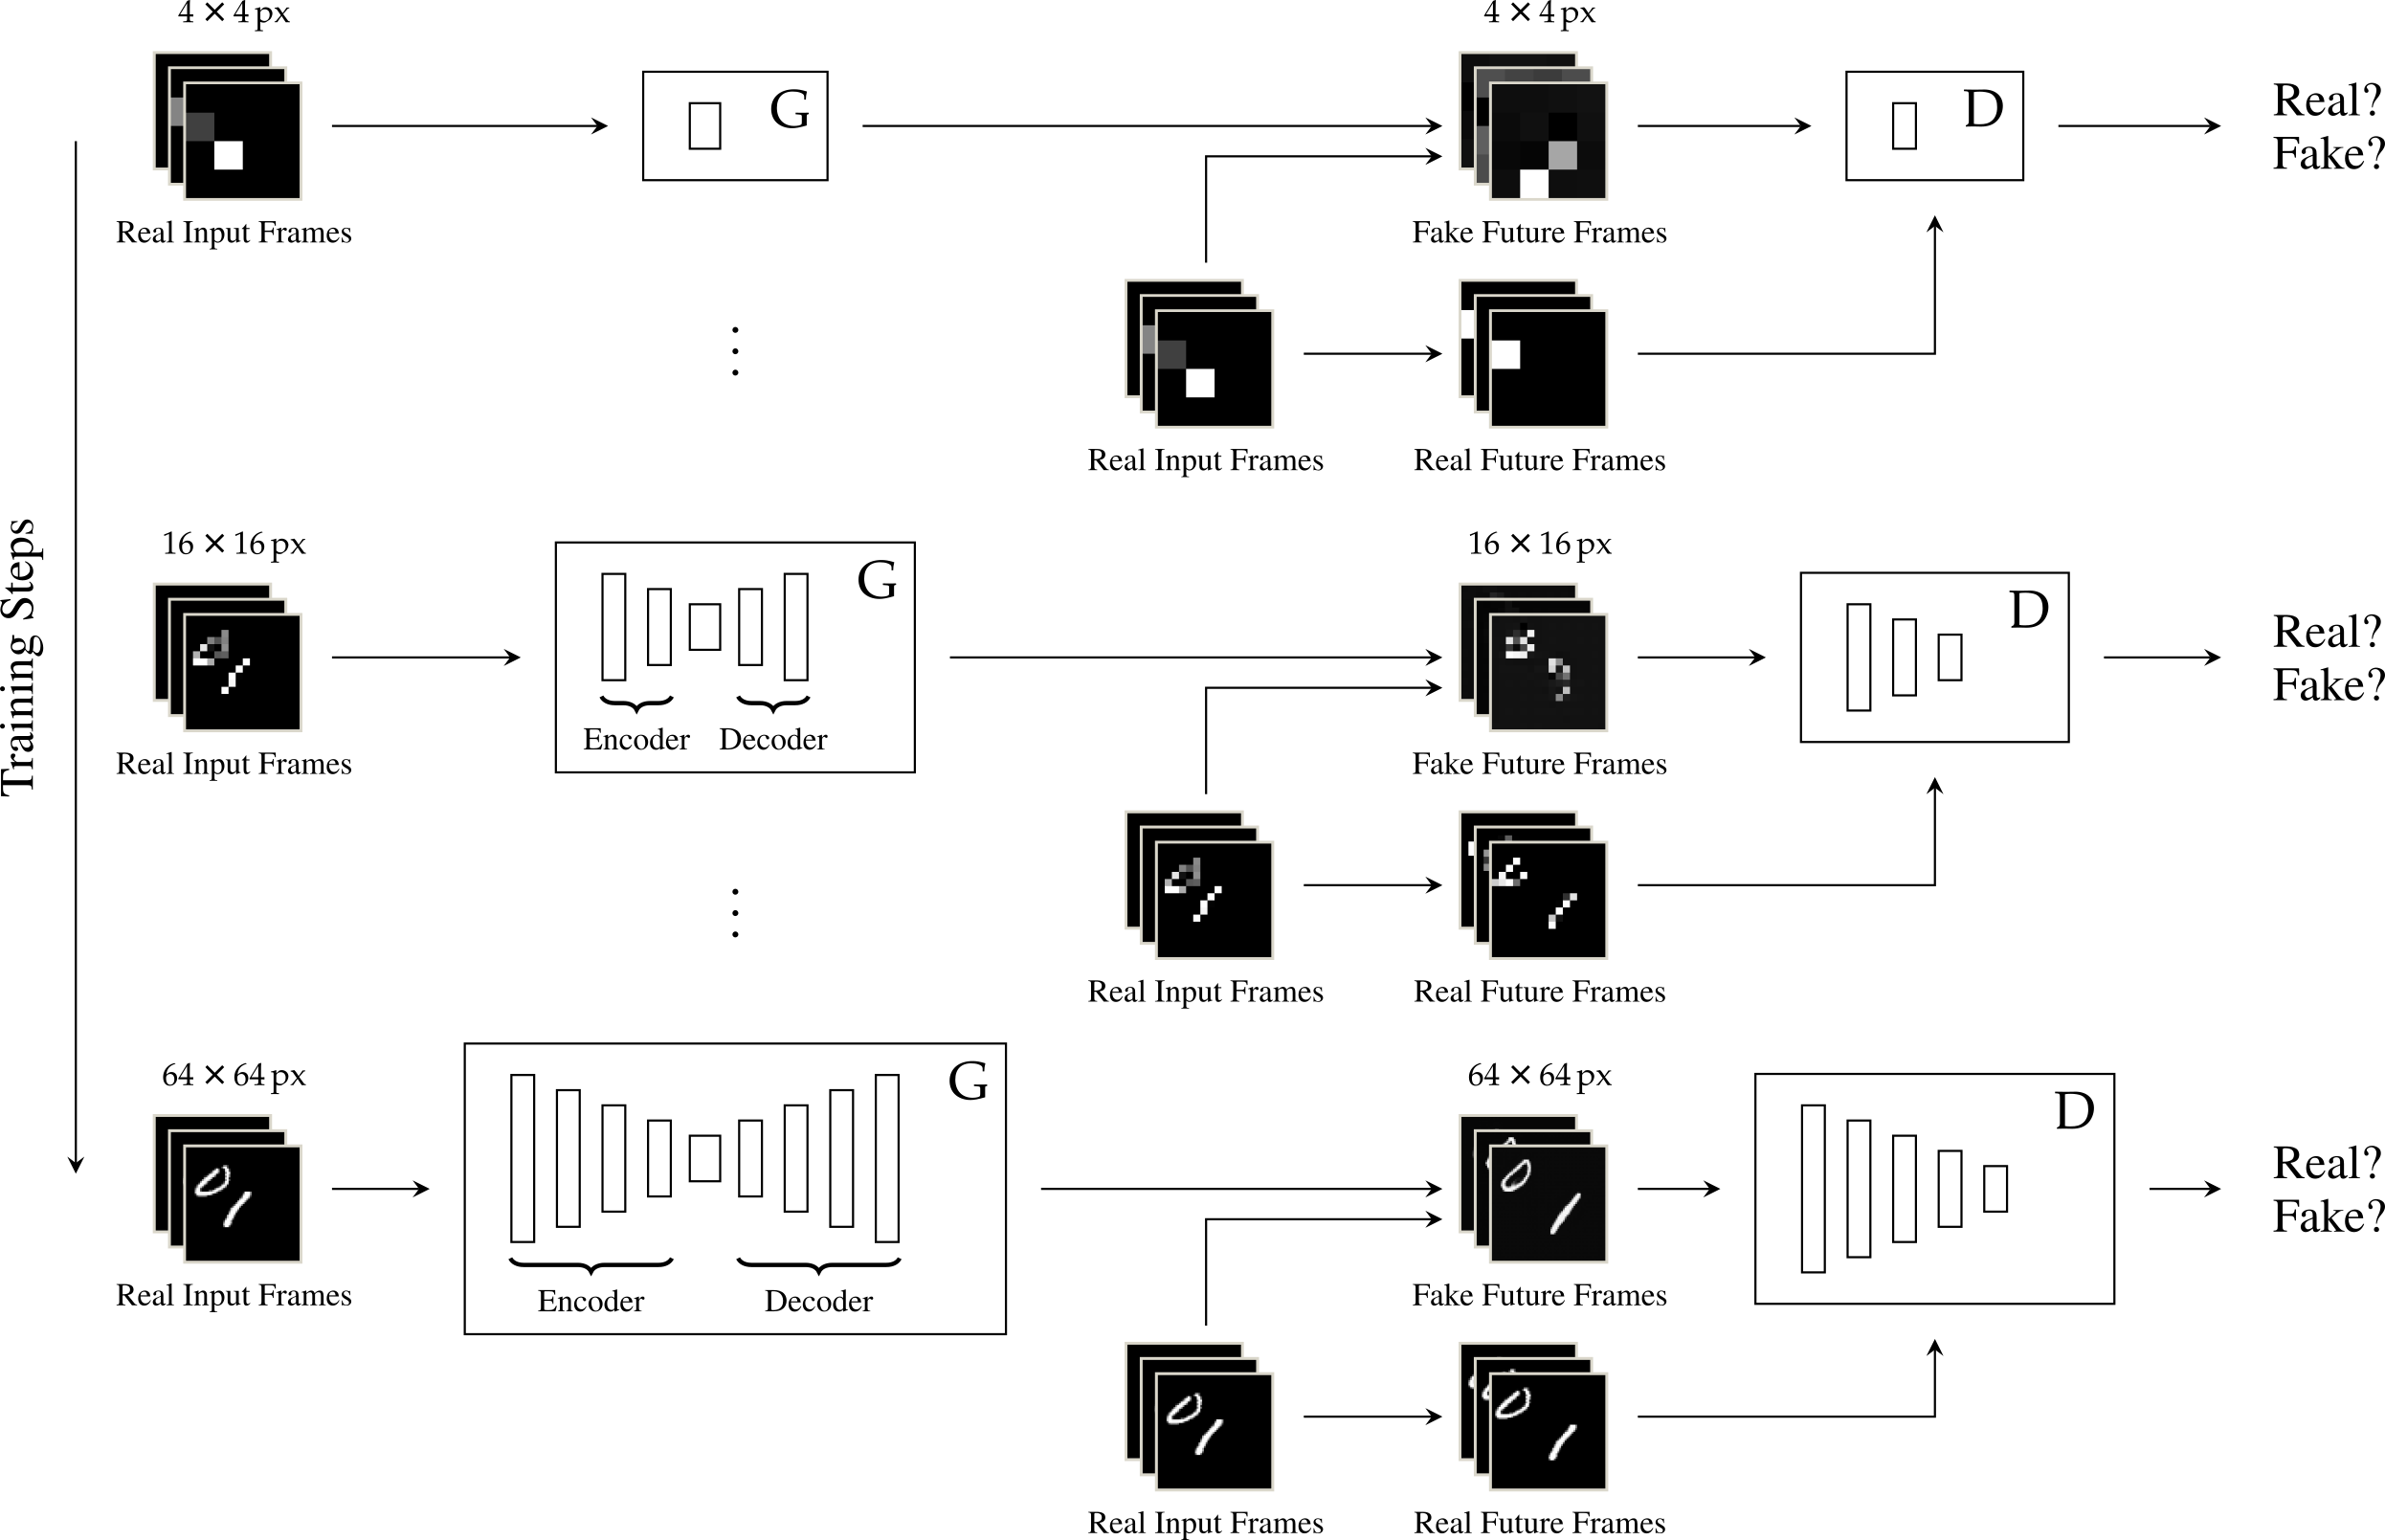
\includegraphics[width=1\textwidth]{figures/futuregan_arch.png}
% 	\end{center}
% 	\caption{FutureGAN Architecture}
% 	\label{fig:futuregan_arch}
% \end{figure}
%
% \subsection{SAVP}
% \label{subsec:savp}

% \newpage
% \section{Datasets}
% \label{sec:datasets}
%
% The datasets used in this project are 
% Datasets used in video prediction tasks have a wide range, and often include datasets made for other tasks.
%
% \subsection{MovingMNIST}
% \label{subsec:mmnist}
%
% \subsection{KTH}
% \label{subsec:kth}
%
% \subsection{BAIR}
% \label{subsec:bair}

\newpage 
\section{Implementation and Training Details}
\label{sec:details}

Implementation of all model architecture discussed in this report (which can be
found in \href{https://github.com/msc5/junior-iw}{This GitHub repository}) was
carried out using PyTorch \cite{pytorch}, with other utility code for model
training, saving, and organization done using PyTorch-Lightning
\cite{pytorch_lightning}. Code for the each video dataset \codeword{DataLoader}
class was sourced from the \href{https://github.com/edenton/svg}{GitHub
repository} for the implementation of the paper Stochastic Video Generation
with a Learned Prior \cite{svg_dataloaders}. (This was for convenience and to
ensure that data sampled in this project would be the same as the data used in
common video prediction implementations.) The three \codeword{DataLoader}
instances used in the linear sequence prediction experiments are described in
the following section.

The implementation the LSTM cell matches the details described in the previous
sections, with the addition of a final layer which acts on the collected
predictions $\hat{\boldsymbol{Y}}$ in order to map them back into the original
input channel dimension. For the LSTM with linear layers, this was another
linear layer with an input dimension of 64 (the number of hidden channels used
in all models) and an output dimension of 1. For the ConvLSTM, this was a 3D
convolution with a kernel size of $(3, 3, 3)$, `same' padding, and an output
channel dimension of 1 or 3, depending on whether the dataset used was
black-and-white or in RGB color.

Each model was trained using Stochastic Gradient Descent (SGD) with a learning
rate of 0.001 on batches of size 4 for the video datasets and 64 for the
sequence datasets. The input sequence length and predicted sequence lengths for
the video and sequence datasets were 10 and 10 frames, and 25 and 25 points,
respectively.

\newpage
\section{Datasets}
\label{sec:datasets}

\subsection{Sequence Datasets}
\label{subsec:sequence_datasets}

The main experimental procedure carried out in this report is the training and
testing of the Convolutional LSTM model on the MovingMNIST, KTH, and BAIR
datasets, however, in order to more gain a more robust understanding of LSTM
features and limitations, as well as to debug the training mechanisms in a much
simpler setting, it was useful to first test a Linear LSTM model on
one-dimensional sequential data before moving fully to video prediction. Three
datasets of this type were implemented: a dataset consisting of generated sin
waves with random frequency and phase offset, a dataset consisting of NASDAQ
close price data from 8 tech companies, and a dataset consisting of randomly
generated points. The choice of these datasets were intended to each test the
model with a varying degree of stochasticity, the sin waves being the most
deterministic, or predictable, the random points being the most stochastic, or
random, and the stock price data hopefully being somewhere in between. Some
specific details about these datasets are described in the following sections.

\subsubsection{GeneratedSins}
\label{subsubsec:generatedsins_dataset}

This dataset was generated by simply plotting a sinusoid function:

\begin{equation}
	\boldsymbol{X} (t) = \boldsymbol{Y} (t) = \frac{1}{2} ( \sin (\alpha t + \beta) + 1)
	\label{eq:generated_sins}
\end{equation}

With random $\alpha$ and $\beta$. This results in a sin wave with a random
frequency and phase offset plotted within the range $[0, 1]$. Although this
dataset has random features, once the sin wave is detected and learned by the
model, it should be relatively easy to predict, since sin waves are perfectly
periodic. $\boldsymbol{X}$ consists of 25 data points evaluated from $[0,
0.5)$, and likewise, $\boldsymbol{Y}$ consists of 25 data points from $(0.5,
1]$. In sum, the train split consists of 22000 samples, and the test set
consists of 7000. 

\subsubsection{GeneratedNoise}
\label{subsubsec:generatednoise_dataset}

This dataset was generated by using pytorch's random tensor function
\codeword{torch.rand()}, which generates a tensor of specified dimensions,
where each entry is a float uniformly distributed within $(0, 1)$. To make this
data a little easier to view, this data was then smoothed using
\codeword{scipy.ndimage.filters.gaussian_filter1d()} function, which convolves
the signal with a 1-dimensional gaussian kernel with $\sigma = 1$. The train
split consists of 22000 samples, and the test set consists of 7000.

\subsubsection{Stocks}
\label{subsubsec:stocks_dataset}

This dataset was sourced using Alpha Vantage \cite{alpha_vantage}, a free
online stock price API. Close price data is provided from the past two years
for the NASDAQ tickers `GOOGL', `MSFT', `TSLA', `AAPL', `AMZN', `NVDA', `FB',
and `AMD'. This data is normalized by subtracting the minimum and dividing by
the maximum for each sequence individually, such that each sequence pulled from
the dataset lies within $(0, 1)$, and is therefore comparable to the other
datasets. The train split consists of 22277 samples, and the test set consists
of 7312 samples.

\subsection{Video Datasets}
\label{subsec:video_datasets}

The video datasets chosen in this report are MovingMNIST \cite{mmnist_dataset},
KTH \cite{kth_dataset}, and BAIR \cite{bair_dataset}. All datasets were
downsampled to $64 \times 64$ frames, with MovingMNIST and KTH having one
channel dimension and BAIR having three. Each sequence sampled from these
datasets was trimmed to 20 frames total, with the first 10 being the input to
the model and the last 10 being the ground truth label, representing the
duration the model was tasked to predict.

The MovingMNIST consists of a pair of white MNIST \cite{mnist_digits} bouncing
around over a pure black background. The digits in the train split of
MovingMNIST are chosen randomly from the training MNIST digits split, and
likewise for the testing split.

The KTH dataset consists of one person (or zero) against a mostly solid
background (either indoors or outdoors) performing one of six actions (walking,
jogging, running, boxing, hand waving and hand clapping).

The BAIR dataset consists of a robot arm pushing around a collection of
children's toys across a table top. 

\newpage
\section{Experiments}
\label{sec:experiments}

% \begin{table}
% 	\caption{Summary of Main ConvLSTM Results}
% 	\label{tab:results_summary}
% 	\begin{center}
% 		\begin{tabular}{ l l l l }
% 			\textbf{Dataset} & \textbf{Number of layers} & \textbf{Number of Parameters} & \textbf{Test MSE Loss} \\
% 			MovingMNIST & \\
% 			KTH & \\
% 			BAIR
% 		\end{tabular}
% 	\end{center}
% \end{table}

When researching and implementing a prediction model of any sort, it is
important to consider that certain sequences are simply impossible to predict,
and that even if the model were ``perfect'' by human standards, it would still
fail to perform this task perfectly. The interesting question here is not
whether the model will be able to achieve a certain accuracy in predicting the
sequences but rather where or how exactly will it fail? And where it does fail,
which features of the model's architecture and methodology are to blame?

All these questions lead directly into one of the major concerns in video
prediction research, which is that the task is inherently hard to judge
\cite{video_prediction_survey}, particularly that pixel-wise loss functions,
such as the Mean Squared Error (MSE) function used to train this model, cause
models to prefer blurry results that average out multiple possibilities for the
next time step rather than a single, clearer image that could be very wrong
using pixel-wise metrics. Models trained in this way are not directly learning
to produce images but merely to appease the loss function, and these results
may not be as clear or useful to humans, and are therefore not preferred in
research discussion.

% This Linear LSTM was implemented with nearly the same exact architecture as the
% Convolutional LSTM, however with Linear layers in place of convolutions, and as
% a result, a 2D convolution layer as the final step as opposed to 3D. Each time
% it was trained on sequences of length 50, for a total duration of 10 epochs.

\subsection{Sequence Prediction}
\label{subsec:experiment_sp}

The MSE loss was recorded as the model was trained, and a plot of this is shown
in Figure \ref{plt:lstm_train_loss}. In addition, after training was complete,
a plot was generated of the model's average loss on the test split as the
predicted sequence progresses, which is shown in Figure
\ref{plt:lstm_seq_loss}. The average loss over the whole test split is shown in
Table \ref{tab:lstm_avg_loss}.

\begin{figure}[H]
	\begin{center}
		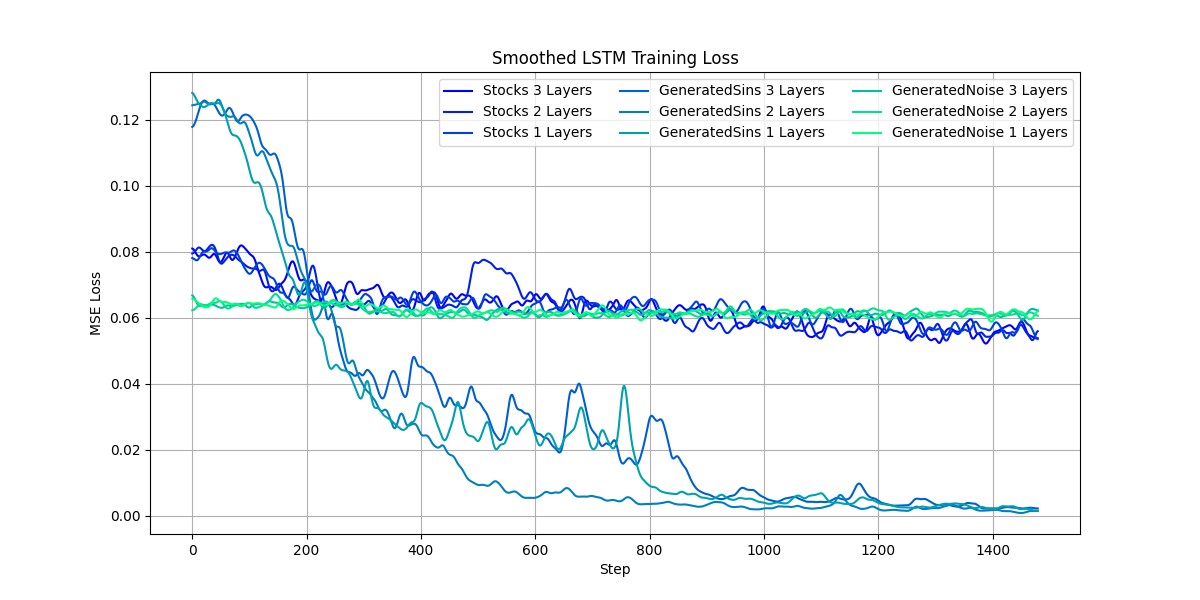
\includegraphics[width=1\textwidth]{plots/lstm_train_loss.png}
	\end{center}
	\caption{LSTM Training Loss on GeneratedSins, GeneratedNoise, and Stocks
	Datasets for Models with Varying Number of Cell Layers}
	\label{plt:lstm_train_loss}
\end{figure}

\begin{figure}[H]
	\begin{center}
		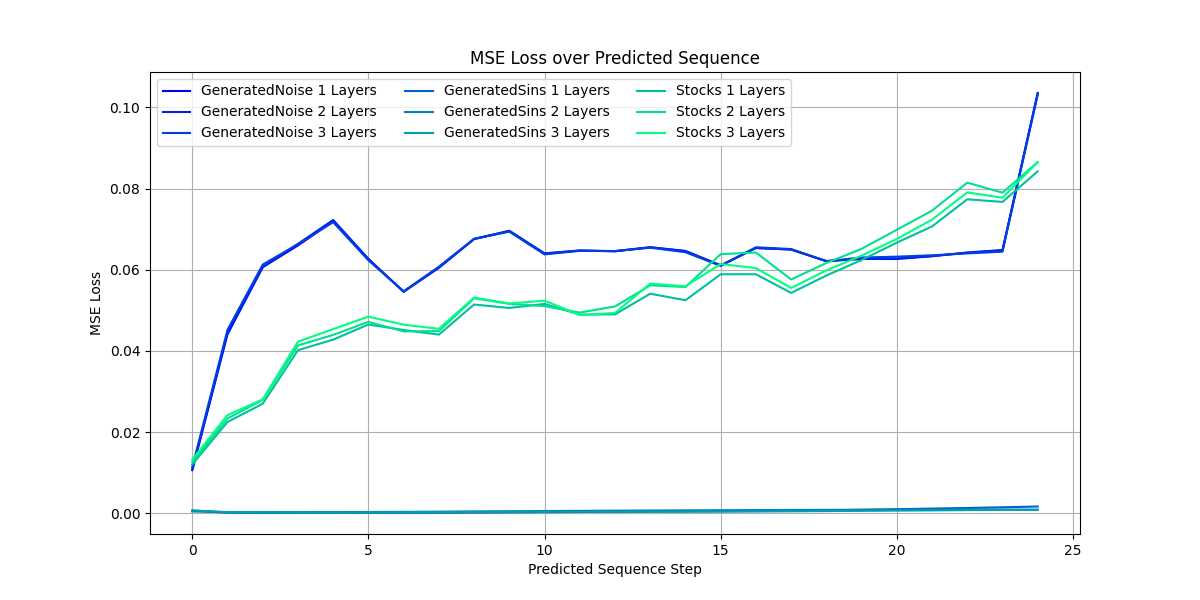
\includegraphics[width=1\textwidth]{plots/lstm_seq_loss.png}
	\end{center}
	\caption{LSTM Test Loss over Predicted Sequence Steps for GeneratedSins, GeneratedNoise, and Stocks Datasets for Models 
	with Varying Number of Cell Layers}
	\label{plt:lstm_seq_loss}
\end{figure}

\begin{table}[H]
	\caption{LSTM Average Test Losses vs. Number of Layers}
	\label{tab:lstm_avg_loss}
	\begin{center}
		\begin{tabular}[c]{ p{0.7in} p{1.3in} p{1.3in} p{1in} }
			\textbf{Layers} & \textbf{GeneratedNoise} & \textbf{GeneratedSins} & \textbf{Stocks} \vspace{0.3em} \\
			\textbf{1}      & \num{5.964e-2}          & \num{4.950e-4}         & \num{5.227e-2}                 \\
			\textbf{2}      & \num{5.967e-2}          & \num{6.298e-4}         & \num{5.431e-2}                 \\
			\textbf{3}      & \num{5.961e-2}          & \num{4.804e-4}         & \num{5.381e-2}
		\end{tabular}
	\end{center}
\end{table}

Additional test inferences for each dataset are shown in the Appendix Section
\ref{subsec:additional_sequence_inferences}.

\subsubsection{GeneratedSins}
\label{subsubsec:generated_sins}

The results shown in the previous figures confirm this dataset to be the most
predictable of the three. This can be observed in the plot of training losses
in Figure \ref{plt:lstm_seq_loss}, which shows that models trained on
GeneratedSins data generally decreased the most over training out of the three,
and in the plot of average test losses over the predicted sequence in Figure
\ref{plt:lstm_train_loss}, which shows that GeneratedSins led to the most
accurate predictions over longer sequences by far. Additionally, Table
\ref{tab:lstm_avg_loss} shows that the average test loss from this dataset was
only \num{e-2} times the average losses of the others. A Test inference of a
2-layer LSTM model trained on this dataset with the ground truth sequence
underlaid is shown in Figure \ref{inf:lstm_sins_inference}. 

\begin{figure}[H]
	\centering
	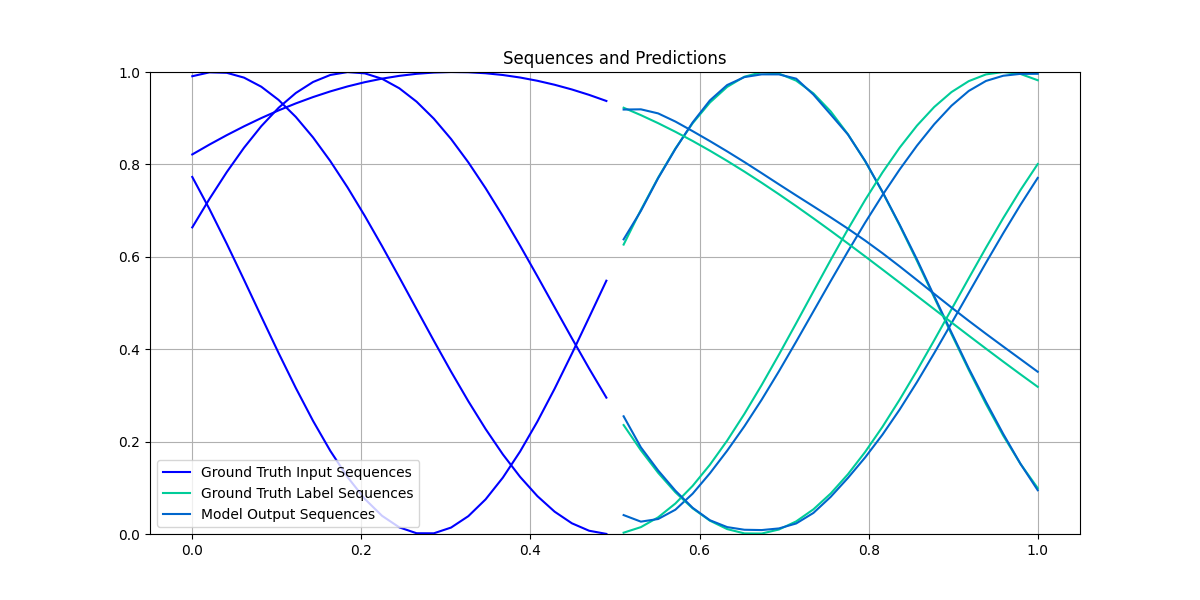
\includegraphics[width=1\textwidth]{inferences/sins/3layer_s11.png}
	\caption{4 LSTM Inferences on Test Split of GeneratedSins Dataset}
	\label{inf:lstm_sins_inference}
\end{figure}

As clean and impressive as these predictions are, however, they are not
perfect, and still decrease in accuracy as the sequence progresses. While the
errors are minor in this demonstration, the shortcoming reveals a pretty major
property of the Seq2Seq architecture (and all sequence prediction
architectures, not just Seq2Seq), which is that in general, predictions will
tend to decrease in accuracy as they become longer. In most situations, this is
because real data is at least some part stochastic, meaning that, as time goes
on, a sequence can have many possible outcomes, and the state of the sequences
at any far-off point in time is a composition of all the previous random events
that take place. In this situation, however, a feature of the Seq2Seq modeling
is most likely the culprit (excluding possible training and implementation
errors), since there is \textit{no} inherent stochasticity of a sin wave, that
is, it is not a random process at all and once it is established at any point
in time it will continue in that way forever. 

In this situation, when the model feeds each LSTM cell's output directly back
into itself as an input for the next time step in order to generate the full
sequence (See Figure \ref{fig:seq2seq_arch}), if any prediction is off by a
tiny amount, then the next prediction will likely share and even increase that
error. While it is likely that this is the phenomenon causing the majority of
the error in this situation, the small initial errors are most likely due to
incomplete convergence of the model, since the training and test set should
theoretically approach the same distribution as more samples are drawn.

\subsubsection{GeneratedNoise}
\label{subsubsec:generated_noise}

This dataset, in contrast, was nearly impossible for the model to learn
satisfactorily, as evidenced by the training loss plot shown in Figure
\ref{plt:lstm_train_loss} which is essentially flat. Additionally, over the
test sequences on average in Figure \ref{plt:lstm_seq_loss}, the model
increases most rapidly in error as the prediction increases in duration. While
this result is somewhat expected for this dataset, it is still concerning that
the model is capable of predicting any amount of a random signal for any
duration. The answer to this question lies in the details of the dataset
implementation, specifically that the points are not purely random after all;
they become slightly cross-correlated after being smoothed by the gaussian
filter, due to the convolution action which sums neighboring points. A batch of
test inferences showcasing this phenomenon is shown in Figure
\ref{inf:lstm_noise_inference}.

As for the model implementation and architecture, one important aspect of the
results on this dataset stands out, which is that the model predicts nothing
but a flat line centered at 0.5 after these initial predictions. This may seem
like an uninteresting result, but what it shows is fundamentally the same issue
that will cause blurry predictions in actual video predictions, and this is one
of the current challenges discussed in video prediction research
\cite{video_prediction_survey}.

To analyze the issue here, it is necessary to closely evaluate the loss
function used in training this model:

\begin{equation}
	\text{MSE} = \frac{1}{n} \sum_{i = 1}^n ( Y_i - \hat{Y}_i )^2
	 \label{eq:mseloss}
\end{equation}

The issue with this loss function is that it assumes that the underlying data
distribution is Gaussian. Here, it is nearly the case that $X, Y \sim U(0, 1)$,
and the expected value of the uniform distribution $\mu = \frac{1}{2} (1 - 0) =
0.5$ will minimize the MSE loss, even if $\mu$ itself has very low probability
of occurring on its own right. This feature of pixel-wise loss functions has
negative side-effects for video prediction, since the mean prediction does not
usually yield very realistic frames, and these types of predictions are not
useful to humans.
 
\begin{figure}[H]
	\centering
	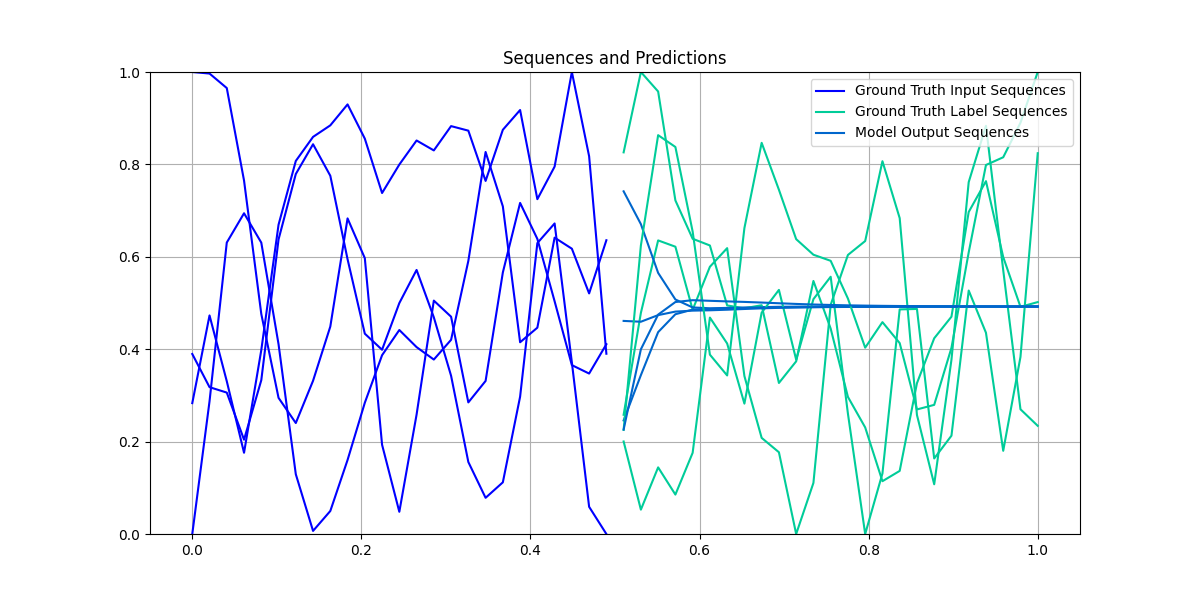
\includegraphics[width=1\textwidth]{inferences/noise/3layer_s13.png}
	\caption{4 LSTM Inferences on Test Split of GeneratedNoise Dataset}
	\label{inf:lstm_noise_inference}
\end{figure}

% The methods used to limit this negative effect are to use adversarial training,
% more complex loss functions, or modeling the prediction using probability \cite{}.

\subsubsection{Stocks}
\label{subsubsec:stocks}

Prior to performing this experiment, it was difficult to hypothesize how the
LSTM model would perform on the stock price dataset, partly because the author
knows very little about finance in general, but also because if it could be
done reliably, then it would not be hard to make a lot of money very easily!
However, from the previous experimentation with the GeneratedNoise dataset, it
was reasonable that stock data points should be more cross-correlated between
neighboring points, since stock prices should have some underlying
predictability, even if it is minor.

In practice, the results of testing the model on this dataset showed some
interesting phenomenon and differences when compared to GeneratedNoise.
Firstly, the model does not just predict the mean for every sequence with this
dataset, instead, it attempts to fit each line individually, as can be seen in
Figure \ref{inf:lstm_stocks_inference}. In addition, the average test loss over
this dataset shown in Figure \ref{plt:lstm_seq_loss} reveals that the
prediction error does not decrease as quickly as with GeneratedNoise, and the
training loss plot shown in Figure \ref{plt:lstm_train_loss} shows that the
overall decrease in loss over the stocks dataset was greater than for
GeneratedNoise. These results show that the model does learn something from the
stocks sequences, even though they are, at first glance, just as random and
unpredictable as the random noise.

\begin{figure}[H]
	\centering
	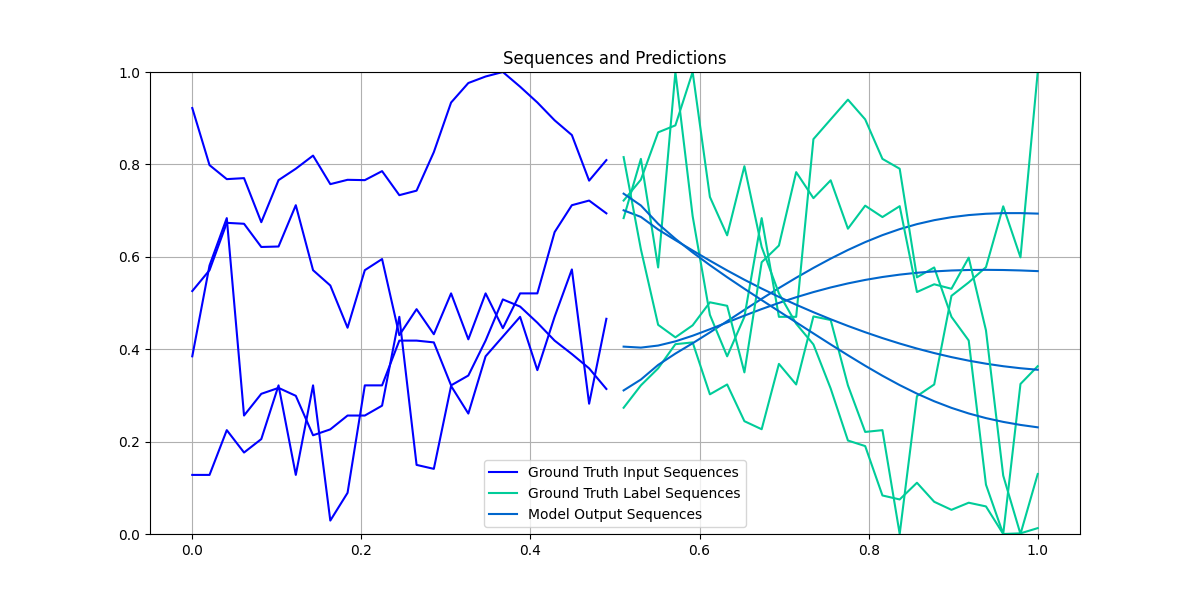
\includegraphics[width=1\textwidth]{inferences/stocks/3layer_s31.png}
	\caption{4 LSTM Inferences on Test Split of Stocks Dataset}
	\label{inf:lstm_stocks_inference}
\end{figure}

While some of the predictions from this dataset are impressive, however, and
seem to almost approximate the trajectory of the stock price, a good amount of
them are also mostly wrong, and even seem to diverge from the ground truth
label completely. From a qualitative perspective, these predictions do not seem
accurate enough to make any serious decisions off of, however, it would be very
interesting to test the performance of this model in making trading decisions
as a future experiment.

\newpage
\subsection{Video Prediction}
\label{subsec:experiment_vp}

Now on to the focus of this project, which is to use a variation of the
previously-used model equipped with convolution in order to predict the
continuation of video sequences. 
 
\begin{figure}[H]
	\centering
	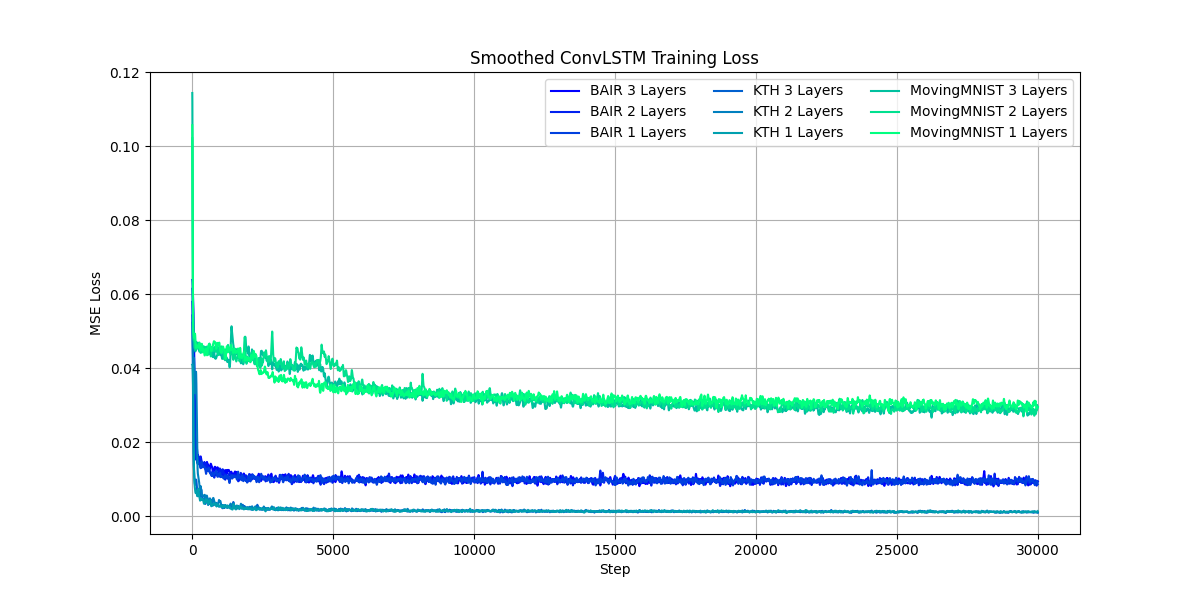
\includegraphics[width=1\textwidth]{plots/convlstm_train_loss.png}
	\caption{ConvLSTM Training Loss on MovingMNIST, KTH, and BAIR Datasets for Models with Varying Number of Cell Layers}
	\label{plt:convlstm_train_loss}
\end{figure}

\begin{figure}[H]
	\centering
	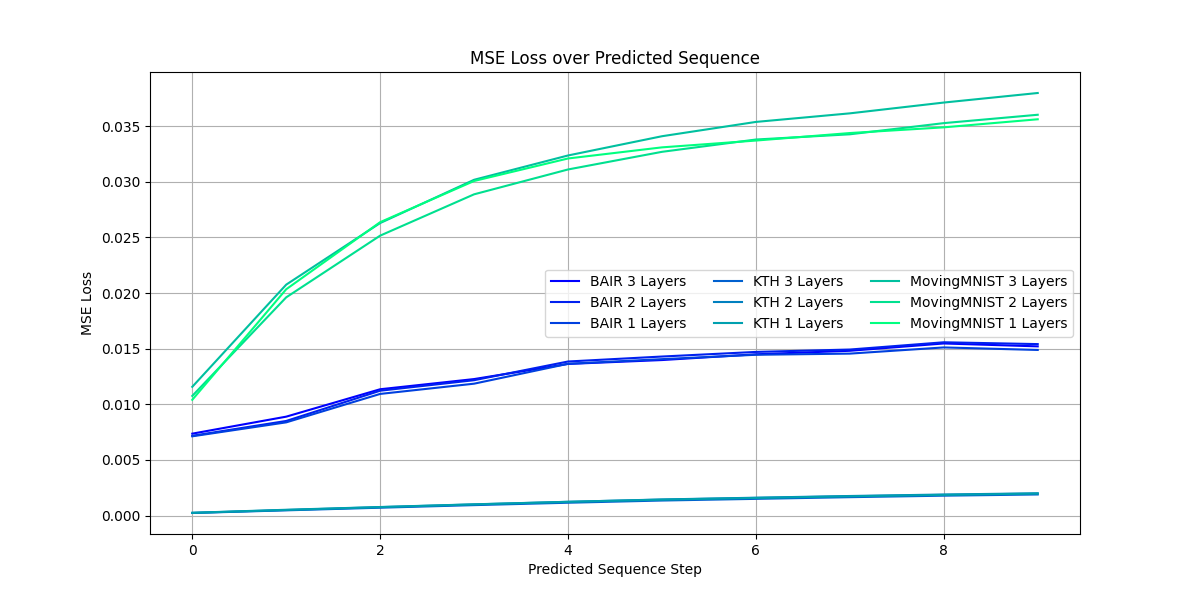
\includegraphics[width=1\textwidth]{plots/convlstm_seq_loss.png}
	\caption{ConvLSTM Test Loss over Predicted Sequence Steps on MovingMNIST, KTH, and BAIR Datasets for Models with Varying Number of Cell Layers}
	\label{plt:convlstm_seq_loss}
\end{figure}

As before, this model's training loss over the three video datasets
MovingMNIST, KTH, and BAIR are shown in Figure \ref{plt:convlstm_train_loss},
and the average test loss plotted over the prediction sequence steps for each
dataset and number of cell layers is shown in Figure
\ref{plt:convlstm_seq_loss}. Additionally, the average test loss is shown in
Table \ref{tab:convlstm_avg_loss}.

\begin{table}[H]
	\caption{ConvLSTM Average Test Losses For Each Dataset and Number of Layers}
	\label{tab:convlstm_avg_loss}
	\begin{center}
		\begin{tabular}[c]{ p{0.7in} p{1.3in} p{1in} p{1in} }
			\textbf{Layers} & \textbf{MovingMNIST} & \textbf{KTH}    & \textbf{BAIR} \vspace{0.3em} \\
			\textbf{1}      & \num{1.249e-02}      & \num{1.233e-03} & \num{2.910e-02}              \\
			\textbf{2}      & \num{1.278e-02}      & \num{1.239e-03} & \num{2.876e-02}              \\
			\textbf{3}      & \num{1.274e-02}      & \num{1.163e-03} & \num{3.019e-02}
		\end{tabular}
	\end{center}
\end{table}

Additional test inferences for each dataset are shown in the Appendix Section
\ref{subsec:additional_video_inferences}.

\subsubsection{Moving MNIST}
\label{subsubsec:mmnist}

The model's inferences on the MovingMNIST were annoyingly mixed, with some
results being quite clear, such as the one shown in
\ref{inf:convlstm_mmnist_inference_1}, and others being much more muddled and
blurry, such as the one shown in \ref{inf:convlstm_mmnist_inference_3}. Since the
MovingMNIST dataset has elements of predictability (for example, digits bounce
off the walls in a predictable way and move at a constant velocity) the
expectation was that this dataset would be easy for the ConvLSTM model to
learn, however, the training loss plot in Figure \ref{plt:convlstm_train_loss}
and the average test sequence loss in Figure \ref{plt:convlstm_seq_loss} show
that this dataset was the most difficult of the three. 

As to why this is the case, it could be a combination of several factors: poor
bias learning, occlusion, or model depth and training time limitations. 

For the first reason, it is important to look at the ways in which MovingMNIST
is unique to the other datasets, for example, it is extremely bimodal, and
pixel intensity values densely cluster around 1 and 0, or white and black, as
they appear in images. Although the LSTM architecture (Figure \ref{fig:lstmcell_arch})
includes a bias term in its weights, the bias needed here is not a simple
pixelwise correction, it is a correction term needed for each frame as the
digits bounce around. While a bias term such as the one included in the vanilla
LSTM cell implementation is capable of correcting the image predictions to be
mostly black, for example, it is not capable of learning that the pixels in
each digit as they bounce around should be white, since the bias terms are
constant over the entire prediction. Thus, the model struggles to produce such
black-and-white predictions.

\begin{figure}[H]
	\begin{center}
		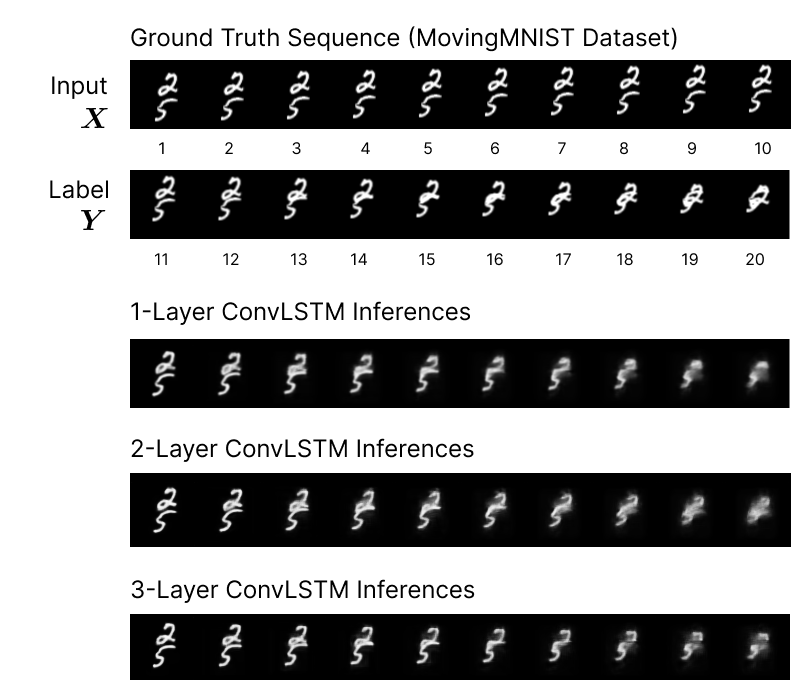
\includegraphics[width=1\textwidth]{inferences/mmnist/mmnist_inferences_1.png}
	\end{center}
	\caption{Convolutional LSTM Inference on MovingMNIST dataset}
	\label{inf:convlstm_mmnist_inference_1}
\end{figure}

While the second reason doesn't account for the high training loss directly,
since occlusion is only present in about half of the sequences and even then
isn't a major factor in most cases, it does increase the underlying complexity
of the dataset to some degree. This, combined with the third reason, could also
be major contributors to the poor prediction accuracy in this case, since the
model was only able to train over 10 epochs due to time and computing power
constraints. Additionally, the dataset is generated on the fly from the MNIST
digits dataset, so it would be easily possible to train a deeper model along
with many more generated sequences in future work.

The dataset creators were able to achieve a much better accuracy using a
different model architecture, an LSTM Autoencoder \cite{mmnist_dataset}.

\begin{figure}[H]
	\begin{center}
		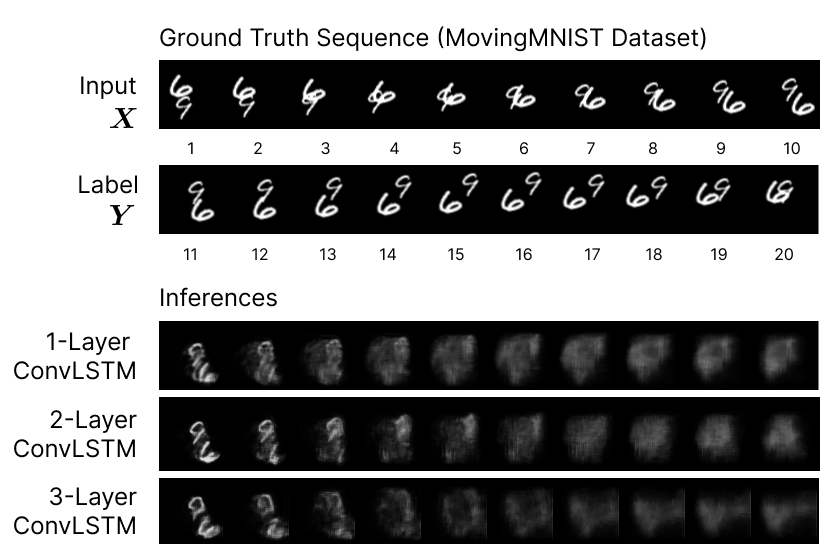
\includegraphics[width=1\textwidth]{inferences/mmnist/mmnist_inferences_3.png}
	\end{center}
	\caption{Convolutional LSTM Inference on MovingMNIST dataset}
	\label{inf:convlstm_mmnist_inference_3}
\end{figure}

\subsubsection{KTH}
\label{subsubsec:kth}

The ConvLSTM model trained and tested best on the KTH dataset out of the three,
as the loss plots in Figures \ref{plt:convlstm_train_loss} and
\ref{plt:convlstm_seq_loss} confirm, and this success led to some of the most
impressive and satisfying predictions in this project. Additionally, the models
trained on the KTH dataset achieved an average test MSE loss of about 10 times
less than the other two.  

The inferences shown in Figure \ref{inf:lstm_kth_inference_1} show a collection
of test predictions done by the model as it trains, and as the model
progresses, it seems to be able to reduce blurring as well as increase
prediction accuracy persistence. Although the train loss does not decrease very
dramatically after the initial decrease in Figure
\ref{plt:convlstm_train_loss}, the predictions become much more clear, showing
that the difference in MSE loss between a blurry image and a clear image that
both roughly approximate the correct prediction is very small.

From a qualitative perspective, this inference is very exciting as it seems to
correctly predict the footsteps of the walking man even during the difficult
stage of occlusion when the legs are superimposed, and for the most part, other
inferences taken from the KTH dataset were similarly detailed. Figure
\ref{inf:lstm_kth_inference_2} shows another inference of similar quality on a
video of a man waving his arms.

\begin{figure}[H]
	\begin{center}
		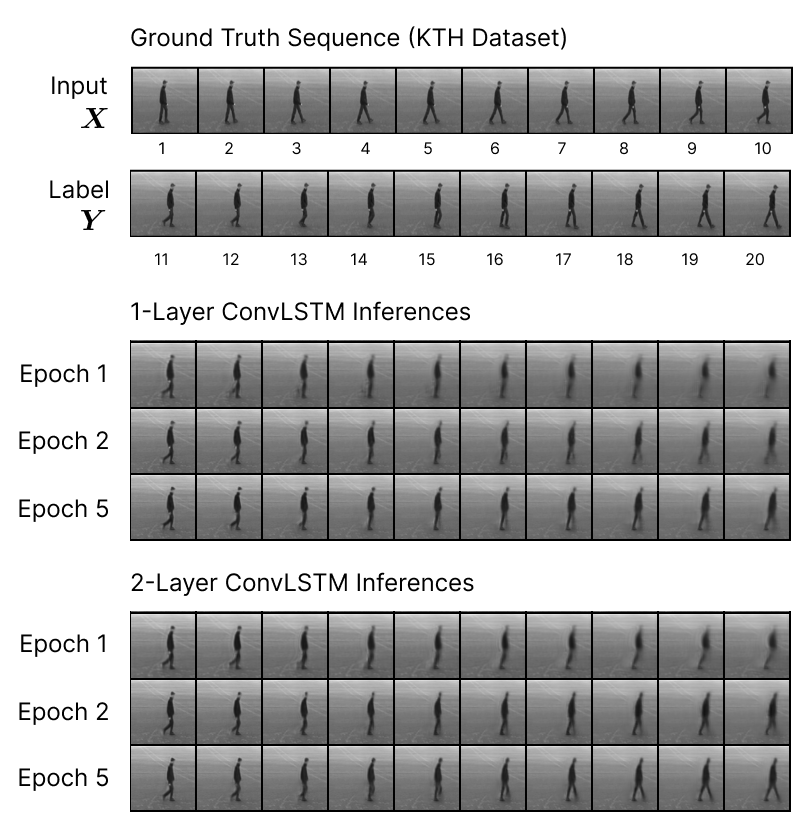
\includegraphics[width=1\textwidth]{inferences/kth/kth_inferences.png}
	\end{center}
	\caption{Convolutional LSTM Inference on KTH dataset (Sample 10)}
	\label{inf:lstm_kth_inference_1}
\end{figure}

This inference (as well as the inferences from the MovingMNIST dataset in
Figures \ref{inf:convlstm_mmnist_inference_1} and
\ref{inf:convlstm_mmnist_inference_3}) also seek to compare the effect of the
number of LSTM cell layers used in the model on the prediction quality, and
this effect seems to be made clear in this example. Compared to the model with
only one layer, the models with 2 and 3 layers are generally able to produce
clearer, more accurate results for this dataset. This detail is also confirmed
by the table of average test losses in Figure \ref{tab:convlstm_avg_loss},
which shows that the 3-layer model had a slightly lower average loss on the KTH
dataset.

\begin{figure}[H]
	\begin{center}
		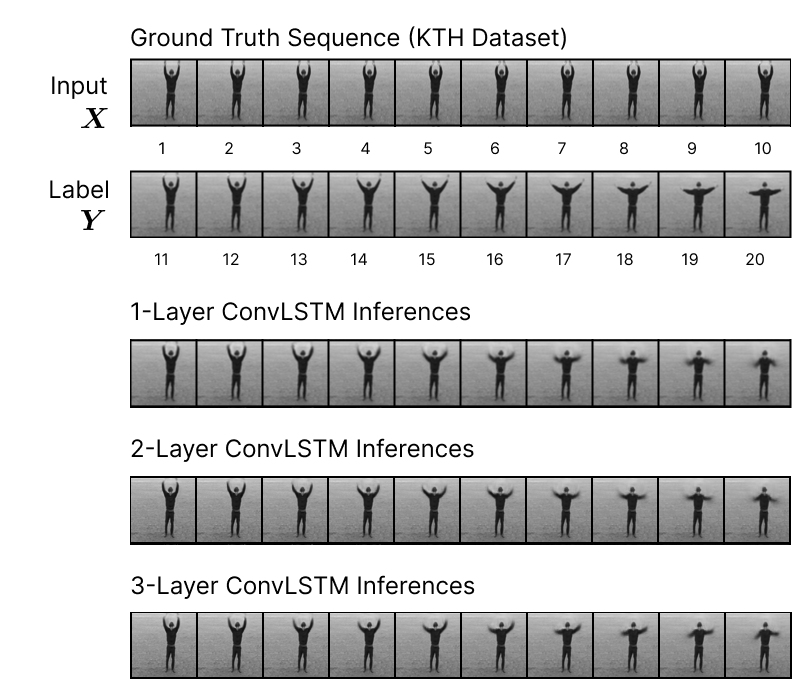
\includegraphics[width=1\textwidth]{inferences/kth/kth_inferences_2.png}
	\end{center}
	\caption{Convolutional LSTM Inference on KTH dataset (Sample 50)}
	\label{inf:lstm_kth_inference_2}
\end{figure}

Although the KTH dataset was the only video prediction dataset in this project
which showed a beneficial effect of adding cell layers, several papers
concluded that more layers should have a positive effect \cite{mmnist_dataset,
seq2seq_original}, and common sense dictates that a model with more parameters
should, in general, be capable of learning a higher-level representation of
training data. Some reasons for why the results in this paper do not match up
with those expectations, therefore, could be that the models trained were
altogether much too small, meaning that there would be little difference
between models with 1, 2, or 3 layers, or that the data used except for KTH is
too complex for such a simple model to predict well at all, which is not an
unlikely conclusion. The most successful predictions seems to come from
adversarial models which incorporate a discrimator in conjunction with a
generator (The Seq2Seq model, for example is a generator) and therefore avoid
blurry predictions as well as some of the other shortcomings of this ConvLSTM
setup (see Section \ref{sec:future_work}).

In short, the reason why adding more layers to the model doesn't simply
increase the accuracy of predictions in this case is most likely because there
are bigger problems at play having to do with fundamental shortcomings of
vanilla LSTMs or severe implementation defects. Therefore section
\ref{sec:future_work} will discuss some popular alternatives and improvements
that could be made to this project's implementation.

\subsubsection{BAIR}
\label{subsubsec:bair}

For engineers, one of the most interesting and immediate applications of video
prediction is to better control robotic movement. While most of this report
discusses video prediction purely from a computer science perspective, it may
actually turn out to be necessary to incorporate research from other domains
such as robotics in order to make meaningful improvements to current computer
science methodologies---after all, as discussed in the introduction, humans
mostly have their own awareness of what will happen in the near future as a
result of observation \textit{and} interaction \cite{human_learning_sequences}.
This motivation may be partly what is behind a growing interconnection between
robotics research and computer vision, as evidenced by growing research in the
field as well as the existence of this dataset and its big brother, RoboNet
\cite{robonet_dataset}, another dataset from Berkeley Artificial Intelligence
Research (BAIR) which contains even more robotic movement videos.

The ConvLSTM model's performance on the BAIR robot pushing dataset used in this
project, however, is mixed. The models trained on this dataset achieved a lower
training loss and test sequence loss than on the MovingMNIST dataset (Figures
\ref{plt:convlstm_train_loss}, \ref{plt:convlstm_seq_loss}), but higher than the KTH
dataset. This could be because the content of the BAIR dataset is more random
than the KTH dataset and the backgrounds are far less uniform, however it is
less directly bimodal, as discussed in Section \ref{subsubsec:mmnist} about the
MovingMNIST sequences.

\begin{figure}[H]
	\begin{center}
		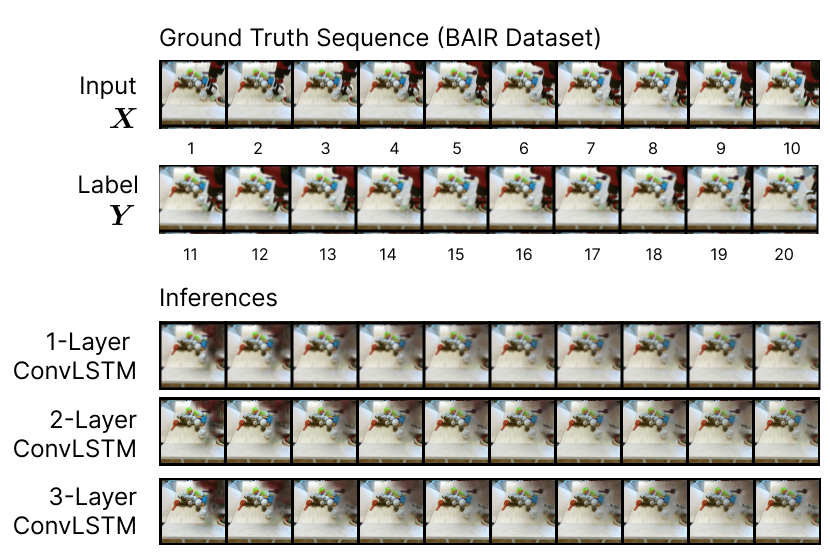
\includegraphics[width=1\textwidth]{inferences/bair/bair_inferences.png}
	\end{center}
	\caption{Convolutional LSTM Inference on BAIR dataset}
	\label{inf:convlstm_bair_inference}
\end{figure}

The inference of the ConvLSTM model shown in Figure
\ref{inf:convlstm_bair_inference} seems to correctly predict the general location
of the robot arm as it moves across the frame, however it is so blurry that it
is hard to tell exactly what the model is fundamentally predicting. While most
of this blurriness likely comes from pixel-wise loss effects (see Section
\ref{subsubsec:generated_noise}), some of it could also be due to the fact that
the robot arm moves very quickly across the frame, and this can be seen in the
ground truth label for this prediction, where the arm disappears from the frame
very suddenly between images 18 and 19. In general, the robot arm in this
dataset does not seem to move at a constant velocity, and it makes many changes
to its trajectory that are hard for a human to predict.

An additional inference is shown in Figure \ref{inf:convlstm_bair_inference_2},
in which it is a little easier to see how the model predicts the general motion
of the arm as it moves to the left edge of the frame. While the BAIR dataset
contains around 40,000 sequences, it also has much more complexity than the
other datasets, since the robot arm is constantly pushing numerous objects
around the frame, and there are countless possible configurations of the arm.
This reason could also help to explain why sequences appear so blurry.

\begin{figure}[H]
	\begin{center}
		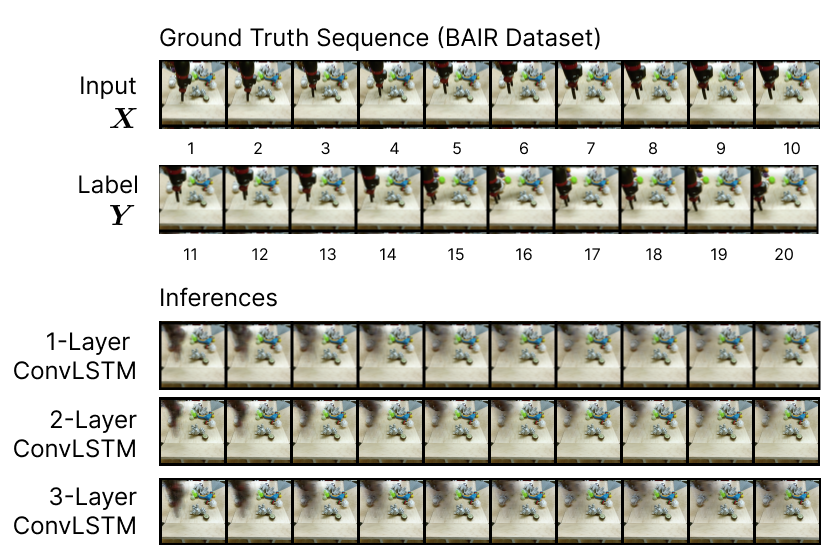
\includegraphics[width=1\textwidth]{inferences/bair/bair_inferences_2.png}
	\end{center}
	\caption{Convolutional LSTM Inference on BAIR dataset}
	\label{inf:convlstm_bair_inference_2}
\end{figure}

\newpage
\section{Future Work}
\label{sec:future_work}

In video prediction research, there are numerous different approaches to video
prediction in addition to the ConvLSTM implementation used here, and some of
them are able to drastically improve on some of the shortcomings encountered in
this project. Batch Normalization, for example, is a well-researched addition
to many computer vision models which can potentially increase LSTM performance,
however, is very difficult to implement with RNNs \cite{batchnorm}. Peephole
connections are an easier improvement to implement, and are described along
with the original presentation of LSTMs \cite{lstm_original}. One of the most
popular and successful alternatives, however, is a Generative Adversarial
Network (GAN), which consists of a generator and a discriminator. A diagram of
the general architecture is shown in Figure \ref{fig:gan_arch}.

A generator used in a GAN consists of mostly the same architecture as a
discriminative neural net, such as the one which might be used for image
classification. While discriminative nets seek to learn the conditional
probability $p(y \mid x)$ of an input $x$ belonging to a particular class $y$;
however, generative nets seek to learn the conditional probability distribution
$p(x \mid y)$ of an input data given the output label, allowing them to make
inferences in the form of ``imagined'' data that might belong to the same
distribution as $x$ \cite{gan_original}. In short, discriminative models would
look at many Van Gogh paintings and fakes in order to learn to differentiate
between them, and generative models would look at many Van Gogh paintings in
order to learn how to paint like Van Gogh. 

\begin{figure}[H]
	\begin{center}
		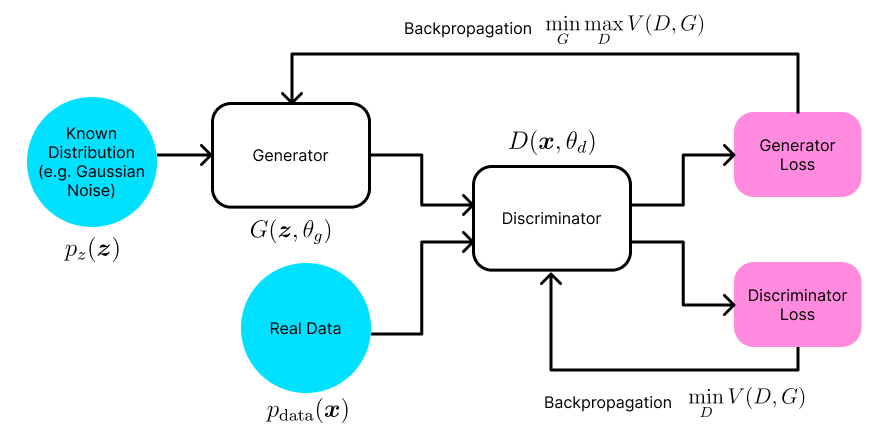
\includegraphics[width=1\textwidth]{figures/gan_arch.png}
	\end{center}
	\caption{FutureGAN Architecture}
	\label{fig:gan_arch}
\end{figure}

In practice, GANs train a generator $G (\boldsymbol{z}, \theta_g)$ which seeks
to learn a mapping from an input noise distribution $p_{\boldsymbol{z}}
(\boldsymbol{z})$ to the targeted data distribution $p_g$ over data
$\boldsymbol{x}$, and a discriminator $D (\boldsymbol{x}, \theta_d)$, which
learns to discriminate between real training samples and generated samples from
$G$. The value function $V(G, D)$, describes the minimax game played between
$G$ and $D$: 

\begin{equation}
	\min_G \max_D V(G, D) = E_{\boldsymbol{x} \sim p_{data} (x)} [ \log (D(x)) ] 
	+ E_{\boldsymbol{z} \sim p_z (\boldsymbol{z})} [ log(1 - D(G(x))) ] 
	\label{eq:gan_value_function}
\end{equation}

The result is a model which is capable of not only generating very good
predictions to minimize pixel-wise loss functions, but also of generating more
predictions which are more likely to occur on their own right. Both FutureGAN
\cite{futuregan} and SAVP \cite{savp} as well as many other video prediction
models which are much more successful than the ConvLSTM model used in this
project use GANs, and so the most clear path for future work in this field is
to implement and test a GAN model and compare its results with the ConvLSTM.

For additional enrichment on the exciting topic of GANs, and as a window into
how the previously described architecture is implemented in practice, a figure
taken from the FutureGAN implementation is shown in Figure
\ref{fig:futuregan_arch}.

\begin{figure}[H]
	\begin{center}
		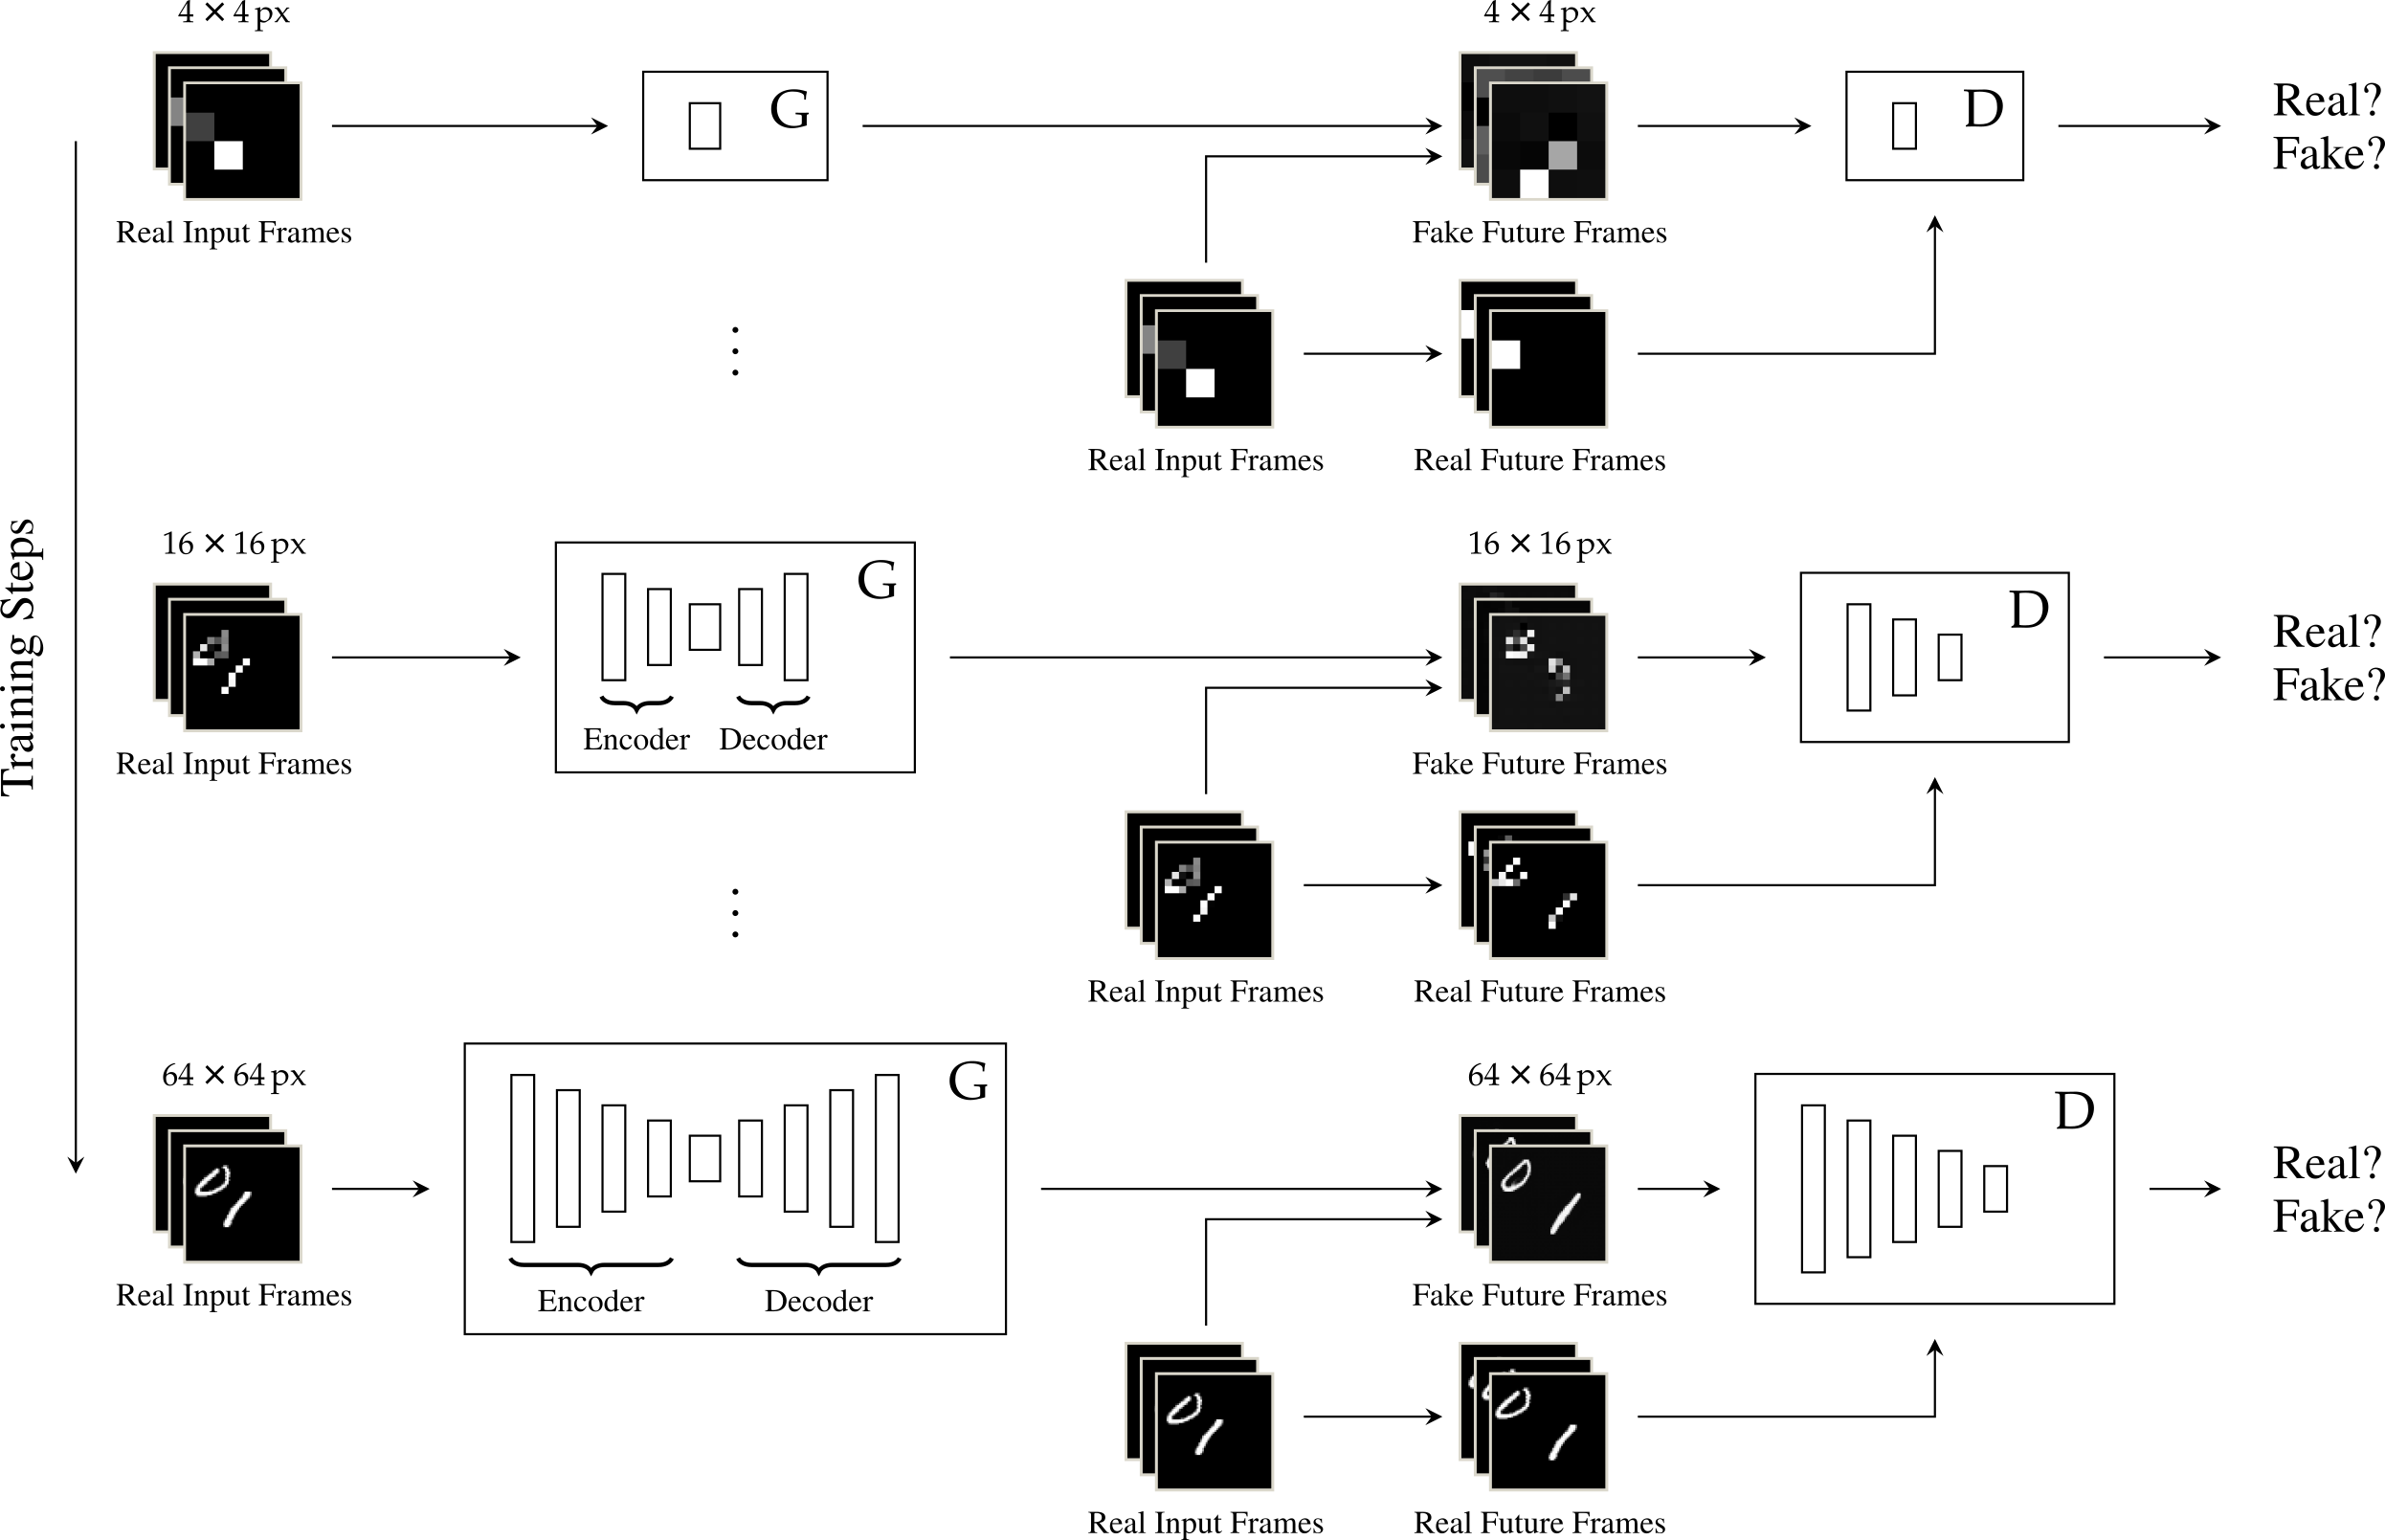
\includegraphics[width=1\textwidth]{figures/futuregan_arch.png}
	\end{center}
	\caption{General GAN Architecture}
	\label{fig:futuregan_arch}
\end{figure}

Note the $G$ and $D$ symbols denoting the model generator and discriminator,
and interestingly, how this model grows in prediction resolution and model
parameters as it trains. FutureGAN was originally singled out as a potential
avenue for future work in this project, but it was discontinued due to time
constraints.

\newpage
\section{Conclusion}
\label{sec:conclusion}

In conclusion, this project represents the successful implementation and
testing of a Seq2Seq LSTM model on several datasets for sequence and video
prediction. In addition, models with varying numbers of cell layers were tested
to determine whether more layers would result in greater prediction accuracy.

In general, the model equipped with linear layers performed extremely well on
the dataset consisting of generated sin waves and was able to predict them with
very high fidelity, although it struggled greatly on the dataset consisting of
generated noise. In addition, it achieved a slight improvement (compared to the
generated noise) on predicting the stock price dataset. The hypothesis that
more cell layers would positively impact model performance held most clearly on
these datasets, as Table \ref{tab:lstm_avg_loss} shows that the models with 3
layers outperformed the models with 1 layer for both the GeneratedNoise and
GeneratedSins datasets. The quantitative results of these experiments are
discussed in Section \ref{subsec:experiment_sp}.

Furthermore, the model equipped with convolutional layers produced mixed
results on the BAIR and MovingMNIST datasets, but performed exceptionally well
on the KTH dataset. One highlight of the experimental results was that each of
the ConvLSTM models with 1, 2, and 3 layers were seemingly capable of
predicting a man's footsteps as he walks through the frame in a sequence
belonging to the KTH dataset. Another promising result from the KTH dataset was
that it was the only dataset of the three for video prediction which confirmed
that more cell layers would equate a greater model performance.

While the results for different numbers of cell layers showed mixed results for
this hypothesis all considered, many of the model's failures as they are
described in each section may contribute to the inconclusiveness of this
testing, such that a dataset was too complex or the model was already too
disadvantaged in predicting samples from a dataset that more layers would not
help in every case. The two datasets which were most successful, however,
GeneratedSins and KTH, both showed improvements with more layers. Since
multiple sources \cite{mmnist_dataset, seq2seq_original} observed that deeper
LSTM networks generally perform better, more exploration is required to examine
the results of this model.

\newpage
\bibliography{main}
\newpage

\newpage
\section{Appendix}
\label{sec:appendix}

\newcommand{\threefig}[6]{
	\begin{figure}[H]
		\centering
		\includegraphics[width=1\textwidth]{#1}
		\caption{#2}
	\end{figure}
	\begin{figure}[H]
		\centering
		\includegraphics[width=1\textwidth]{#3}
		\caption{#4}
	\end{figure}
	\begin{figure}[H]
		\centering
		\includegraphics[width=1\textwidth]{#5}
		\caption{#6}
	\end{figure}
}

\subsection{Additional Sequence Prediction Samples}
\label{subsec:additional_sequence_inferences}

\subsubsection{GeneratedSins}
\label{subsubsec:additional_sins_inferences}

\threefig
{inferences/sins/app_1layer_s29.png}
{4 1-Layer LSTM Inferences on Test Split of GeneratedSins Dataset}
{inferences/sins/app_2layer_s30.png}
{4 2-Layer LSTM Inferences on Test Split of GeneratedSins Dataset}
{inferences/sins/app_3layer_s33.png}
{4 3-Layer LSTM Inferences on Test Split of GeneratedSins Dataset}

\subsubsection{GeneratedNoise}
\label{subsubsec:additional_noise_inferences}

\threefig
{inferences/noise/app_1layer_s29.png}
{4 1-Layer LSTM Inferences on Test Split of GeneratedNoise Dataset}
{inferences/noise/app_2layer_s30.png}
{4 2-Layer LSTM Inferences on Test Split of GeneratedNoise Dataset}
{inferences/noise/app_3layer_s32.png}
{4 3-Layer LSTM Inferences on Test Split of GeneratedNoise Dataset}

\subsubsection{Stocks}
\label{subsubsec:additional_stocks_inferences}

\threefig
{inferences/stocks/app_1layer_s29.png}
{4 1-Layer LSTM Inferences on Test Split of Stocks Dataset}
{inferences/stocks/app_2layer_s30.png}
{4 2-Layer LSTM Inferences on Test Split of Stocks Dataset}
{inferences/stocks/app_3layer_s31.png}
{4 3-Layer LSTM Inferences on Test Split of Stocks Dataset}

\newpage
\subsection{Additional Video Prediction Samples}
\label{subsec:additional_video_inferences}

For each sample shown below, the first row of images is the ground truth input
and label, the second row is the model's prediction, and the third row is the
absolute difference between the label and prediction.

\subsubsection{MovingMNIST}
\label{subsubsec:additional_mmnist_inferences}

\threefig
{inferences/mmnist/app_1layer_s1.png}
{1-Layer ConvLSTM Inference on Test Split of MovingMNIST Dataset}
{inferences/mmnist/app_2layer_s2.png}
{2-Layer ConvLSTM Inference on Test Split of MovingMNIST Dataset}
{inferences/mmnist/app_3layer_s8.png}
{3-Layer ConvLSTM Inference on Test Split of MovingMNIST Dataset}

\subsubsection{KTH}
\label{subsubsec:additional_kth_inferences}

\threefig
{inferences/kth/app_1layer_s7.png}
{1-Layer ConvLSTM Inference on Test Split of KTH Dataset}
{inferences/kth/app_2layer_s12.png}
{2-Layer ConvLSTM Inference on Test Split of KTH Dataset}
{inferences/kth/app_3layer_s14.png}
{3-Layer ConvLSTM Inference on Test Split of KTH Dataset}

\subsubsection{BAIR}
\label{subsubsec:additional_bair_inferences}

\threefig
{inferences/bair/app_1layer_s22.png}
{1-Layer ConvLSTM Inference on Test Split of BAIR Dataset}
{inferences/bair/app_2layer_s32.png}
{2-Layer ConvLSTM Inference on Test Split of BAIR Dataset}
{inferences/bair/app_3layer_s36.png}
{3-Layer ConvLSTM Inference on Test Split of BAIR Dataset}

\end{document}

